\documentclass[a4paper,12pt]{article}

\usepackage[spanish,es-nodecimaldot]{babel}
\usepackage[utf8]{inputenc}
\usepackage[T1]{fontenc}
\usepackage{lmodern}
\usepackage{microtype}
\usepackage{amsmath,amssymb,amsfonts}
\usepackage{geometry}
\geometry{margin=2.5cm}
\usepackage{graphicx}
\usepackage{float}
\usepackage{xurl}
\usepackage{ragged2e}
\usepackage{array}
\usepackage{booktabs}
\usepackage{tabularx}
\usepackage{subcaption}
\usepackage{xcolor}
\usepackage{hyperref}

\hypersetup{
  colorlinks=true,
  linkcolor=black,
  citecolor=black,
  urlcolor=blue,
  pdftitle={Detección y localización de puntos de cambio en trayectorias de difusión anómala},
  pdfauthor={Soulaiman Chair}
}

\newcolumntype{Y}{>{\RaggedRight\arraybackslash}X}
\newcommand{\dd}{\,\mathrm{d}}
\newcommand{\E}{\mathbb{E}}
\newcommand{\Var}{\operatorname{Var}}
\newcommand{\Mset}{\mathcal{M}}
\setlength{\emergencystretch}{2em}
\setcounter{tocdepth}{2}
\setcounter{secnumdepth}{3}

\begin{document}

\begin{titlepage}
\centering
\vspace*{1.8cm}
{\Large \textbf{Trabajo Fin de Máster}\par}
\vspace{1.4cm}
{\huge \textbf{Detección y localización de puntos de cambio en trayectorias de difusión anómala mediante aprendizaje profundo}\par}
\vspace{2cm}
{\Large \textbf{Autor:} Soulaiman Chair\par}
\vspace{0.5cm}
{\Large \textbf{Tutor:} Prof. J. Alberto Conejero\par}
\vspace{1.5cm}
{\large Universitat Politècnica de València\par}
\vfill
{\large Junio de 2026\par}
\end{titlepage}

\section*{Resumen}
\addcontentsline{toc}{section}{Resumen}

La detección de cambios de régimen en trayectorias individuales es un problema central en el análisis de difusión anómala. Una misma ley de escala del desplazamiento cuadrático medio puede surgir de mecanismos estocásticos distintos y, además, las propiedades dinámicas de una trayectoria pueden variar durante la observación. En este trabajo se estudia la detección binaria y la localización temporal de un único punto de cambio en trayectorias sintéticas unidimensionales de longitudes 100 y 200. Los datos combinan cinco modelos utilizados en el \emph{Anomalous Diffusion Challenge}: \emph{annealed transient time motion} (ATTM), \emph{continuous-time random walk} (CTRW), \emph{fractional Brownian motion} (FBM), Lévy walk (LW) y \emph{scaled Brownian motion} (SBM).

La señal de entrada está formada por los incrementos normalizados de la trayectoria. Se comparan cuatro arquitecturas multitarea para $L=100$: LSTM, CNN--LSTM, Transformer y ConvTransformer. Cada red produce una probabilidad de presencia de cambio y una distribución discreta sobre las posiciones temporales admisibles. ConvTransformer ofrece el mejor compromiso global de esa comparación y se evalúa además para $L=200$. En ambas longitudes, las matrices de transición ordenada muestran que el rendimiento depende de qué modelo genera el primer segmento y cuál genera el segundo; los cambios que involucran LW son favorables, mientras que varias transiciones entre ATTM, CTRW y FBM concentran los fallos en $L=200$.

Como análisis complementario se estudia la sensibilidad de ConvTransformer-v2 a cinco inicializaciones aleatorias bajo un régimen reducido de entrenamiento. Tres ejecuciones convergen hacia una solución casi degenerada que declara cambio en prácticamente todas las trayectorias, lo que revela una variabilidad que el resultado principal aislado no permite observar. También se incorpora una referencia clásica basada en PELT, ajustada exclusivamente con validación y evaluada sobre la partición completa de prueba. Las conclusiones se limitan al diseño sintético y a los protocolos efectivamente ejecutados; no se establece una comparación directa con los participantes de AnDi ni una superioridad general de una arquitectura.

\noindent\textbf{Palabras clave:} difusión anómala, punto de cambio, segmentación temporal, aprendizaje profundo, LSTM, Transformer.

\clearpage
\tableofcontents
\clearpage

\section{Introducción}

El movimiento browniano proporciona el modelo de referencia para describir el transporte de una partícula sometida a fluctuaciones rápidas y aproximadamente independientes. Bajo estas condiciones, el desplazamiento cuadrático medio crece de forma lineal con el tiempo. Muchos sistemas físicos y biológicos se apartan de esta ley: macromoléculas en entornos celulares, trazadores en medios desordenados o agentes activos pueden explorar el espacio a un ritmo inferior o superior al browniano. Estos comportamientos se agrupan bajo el término \emph{difusión anómala} y se caracterizan, en primera aproximación, por una ley de potencia con exponente distinto de uno \cite{metzler2000random,metzler2014anomalous}.

La estimación de dicho exponente no identifica de manera unívoca el mecanismo microscópico. Procesos con tiempos de espera pesados, incrementos correlacionados, vuelos persistentes o difusividad dependiente del tiempo pueden producir escalas similares del desplazamiento cuadrático medio. El problema se vuelve más difícil cuando solo se dispone de una trayectoria corta y ruidosa. En ese régimen, los promedios temporales fluctúan, la ergodicidad puede romperse y la información discriminante reside en propiedades locales o correlaciones que un único estadístico global no conserva \cite{metzler2014anomalous,manzo2015review}.

Una dificultad adicional aparece cuando la dinámica no permanece constante durante toda la observación. Una partícula puede pasar de un medio a otro, alternar entre estados de unión y movimiento libre o experimentar una modificación efectiva de la difusividad. La trayectoria deja entonces de estar descrita por un solo régimen. El problema estadístico consiste en decidir si existe una transición y, en caso afirmativo, estimar el instante en el que se produce. Esta formulación enlaza la detección de puntos de cambio con la segmentación de trayectorias de difusión anómala.

El primer \emph{Anomalous Diffusion Challenge} (AnDi) estableció conjuntos simulados y métricas comunes para comparar métodos de estimación del exponente, clasificación del modelo y segmentación \cite{munozgil2021objective}. Sus resultados mostraron la competitividad de los métodos de aprendizaje automático, pero también que ninguna técnica domina todas las longitudes, niveles de ruido y mecanismos generadores. Trabajos posteriores han desarrollado métodos recurrentes capaces de inferir y segmentar trayectorias \cite{bo2019measurement,argun2021classification}, estimadores puntuales de propiedades difusivas \cite{requena2023pointwise} y procedimientos que explotan la incertidumbre predictiva para localizar cambios \cite{seckler2024changepoint}. Por tanto, la elección de una arquitectura debe relacionarse con la estructura estadística de la señal, no solo con su popularidad general.

Este trabajo analiza trayectorias sintéticas compuestas por ATTM, CTRW, FBM, LW y SBM. Se consideran dos escenarios: localización cuando la transición está garantizada y detección conjunta con trayectorias homogéneas. La contribución experimental es una comparación exploratoria de cuatro representaciones neuronales sobre los mismos datos: recurrencia, convolución seguida de recurrencia, autoatención y una combinación de convolución con autoatención. El análisis distingue resultados globales, falsos positivos por modelo homogéneo, falsos negativos por transición ordenada, error de localización y dependencia respecto a la posición temporal del cambio.

Las preguntas de investigación son las siguientes:
\begin{enumerate}
  \item ¿Qué arquitecturas reducen las falsas alarmas sin perder sensibilidad ante cambios reales?
  \item ¿Hasta qué punto las convoluciones locales mejoran la localización en la señal de incrementos?
  \item ¿Cómo depende la dificultad de la dirección del cambio, del modelo generador y de la posición temporal de la frontera?
  \item ¿Qué limitaciones del diseño impiden interpretar las diferencias observadas como una superioridad general de una arquitectura?
\end{enumerate}

La comparación se interpreta como exploratoria: identifica qué conclusiones sostienen los datos disponibles y qué controles faltan para aislar el efecto de la arquitectura.

\section{Fundamentos y estado del arte}

\subsection{De la difusión browniana a la difusión anómala}

Sea $X(t)\in\mathbb{R}^{d}$ la posición de un proceso estocástico. El desplazamiento cuadrático medio de ensamble se define como
\begin{equation}
  \operatorname{MSD}(t)=\E\!\left[\lVert X(t)-X(0)\rVert^2\right].
  \label{eq:msd}
\end{equation}
Para un movimiento browniano homogéneo con coeficiente de difusión $D$, se obtiene $\operatorname{MSD}(t)=2dDt$. En difusión anómala, la ley asintótica se escribe
\begin{equation}
  \operatorname{MSD}(t)\simeq 2dK_{\alpha}t^{\alpha},
  \label{eq:anomalous-msd}
\end{equation}
donde $K_{\alpha}$ es un coeficiente de difusión generalizado. El intervalo $0<\alpha<1$ corresponde a subdifusión; $\alpha=1$, a difusión normal; y $\alpha>1$, a superdifusión. La igualdad del exponente no implica igualdad del proceso: la gaussianidad, la estacionariedad de los incrementos, las correlaciones y la equivalencia entre promedios temporal y de ensamble pueden ser distintas \cite{metzler2000random,metzler2014anomalous}.

En seguimiento de partículas se observa una realización finita $X=(x_1,\ldots,x_L)$. El desplazamiento cuadrático medio promediado en el tiempo para un retardo $\Delta$ es
\begin{equation}
  \overline{\delta^2(\Delta)}=
  \frac{1}{L-\Delta}\sum_{i=1}^{L-\Delta}
  \lVert x_{i+\Delta}-x_i\rVert^2.
  \label{eq:tamsd}
\end{equation}
Esta cantidad es interpretable, pero pierde resolución temporal cuando se calcula sobre la trayectoria completa. Si existe una transición, los dos segmentos contribuyen al mismo promedio. Además, en trayectorias cortas los retardos grandes contienen pocas diferencias; en procesos no ergódicos el promedio temporal no reproduce necesariamente el promedio de ensamble; y el ruido de localización altera la pendiente a retardos pequeños \cite{metzler2014anomalous,manzo2015review}. Estas limitaciones justifican el uso de métodos que operan sobre la secuencia completa o sobre descriptores locales.

\subsection{Modelos generadores}

El conjunto de modelos es
\[
  \Mset=\{\mathrm{ATTM},\mathrm{CTRW},\mathrm{FBM},\mathrm{LW},\mathrm{SBM}\}.
\]
Los cinco procesos comparten una ley anómala para el MSD en determinados rangos, pero la producen mediante mecanismos diferentes.

\subsubsection{Continuous-time random walk}

El CTRW separa la dinámica en saltos espaciales y tiempos de espera. Si los tiempos de espera tienen cola
\begin{equation}
  \psi(\tau)\sim \tau^{-1-\alpha},\qquad 0<\alpha<1,
\end{equation}
su media diverge y aparecen intervalos prolongados de inmovilidad. El número de saltos crece sublinealmente y el MSD escala como $t^{\alpha}$ \cite{montroll1965random,metzler2000random}. En una trayectoria corta, una espera larga puede parecer una frontera; por ello, un detector debe distinguir una fluctuación propia del CTRW de una transición a otro proceso.

\subsubsection{Fractional Brownian motion}

El FBM $B_H(t)$ es un proceso gaussiano autosimilar con parámetro de Hurst $H\in(0,1)$. Su covarianza puede escribirse como
\begin{equation}
  \E[B_H(t)B_H(s)]=\frac{1}{2}\left(t^{2H}+s^{2H}-|t-s|^{2H}\right),
  \label{eq:fbm-cov}
\end{equation}
y $\alpha=2H$ \cite{mandelbrot1968fractional}. Los incrementos son estacionarios pero están correlacionados: son antipersistentes para $H<1/2$ y persistentes para $H>1/2$. Una transición que involucra FBM puede manifestarse como cambio de correlación sin una ruptura clara de amplitud.

\subsubsection{Lévy walk}

En un Lévy walk, la duración de un vuelo y su longitud están acopladas mediante una velocidad finita. Esta restricción evita los saltos instantáneos arbitrariamente largos de un vuelo de Lévy y permite describir transporte superdifusivo con una interpretación física \cite{zaburdaev2015levy}. En los incrementos aparecen intervalos persistentes y excursiones prolongadas. Estas estructuras suelen contrastar con las pausas del CTRW, aunque el ruido y una longitud reducida pueden ocultar el contraste.

\subsubsection{Annealed transient time motion}

ATTM describe un movimiento browniano por tramos con una difusividad $D$ que se renueva después de tiempos de residencia aleatorios. La relación estadística entre $D$ y la duración de cada estado puede generar subdifusión y ruptura de ergodicidad \cite{massignan2014nonergodic}. La heterogeneidad interna es especialmente relevante para este trabajo: una trayectoria homogénea ATTM ya contiene variaciones de difusividad, de manera que no toda modificación local equivale a un cambio de modelo.

\subsubsection{Scaled Brownian motion}

SBM es un proceso gaussiano no estacionario que satisface, en una dimensión,
\begin{equation}
  \dd X(t)=\sqrt{2D(t)}\,\dd W(t),
  \qquad D(t)=\alpha K_{\alpha}t^{\alpha-1}.
  \label{eq:sbm}
\end{equation}
De este modo, $\E[X^2(t)]=2K_{\alpha}t^{\alpha}$, aunque los incrementos no son estacionarios \cite{lim2002selfsimilar,jeon2014scaled}. La evolución gradual de la varianza puede confundirse con una ruptura y hace que el orden de los segmentos influya en la apariencia de la trayectoria.

\begin{table}[htbp]
\centering
\scriptsize
\setlength{\tabcolsep}{2pt}
\begin{tabularx}{0.99\textwidth}{>{\RaggedRight\arraybackslash}p{1.15cm}>{\RaggedRight\arraybackslash}p{2.25cm}>{\RaggedRight\arraybackslash}p{1.95cm}YY}
\toprule
\textbf{Modelo} & \textbf{Mecanismo} & \textbf{Propiedad distintiva} & \textbf{Señal relevante en los incrementos} & \textbf{Riesgo para la detección} \\
\midrule
CTRW & Tiempos de espera pesados & No ergodicidad débil y envejecimiento & Pausas y actividad intermitente & Una espera larga puede simular una frontera \\
FBM & Correlación de largo alcance & Incrementos gaussianos estacionarios & Persistencia o anti-persistencia & El cambio puede residir en la correlación, no en la amplitud \\
LW & Vuelos de duración pesada y velocidad finita & Transporte persistente & Rachas y excursiones largas & Trayectorias cortas pueden contener pocos vuelos informativos \\
ATTM & Difusividad aleatoria por estados & Hetero\-geneidad temporal interna & Cambios locales de escala & Renovaciones internas pueden producir falsos positivos \\
SBM & Difusividad determinista dependiente del tiempo & Incrementos no estacionarios & Varianza que evoluciona gradualmente & Una tendencia suave puede interpretarse como ruptura \\
\bottomrule
\end{tabularx}
\caption{Propiedades cualitativas de los modelos y su relación con la detección de puntos de cambio.}
\label{tab:model-properties}
\end{table}

\subsection{Inferencia automática a partir de trayectorias individuales}

Los primeros enfoques automáticos combinaron descriptores construidos manualmente con clasificadores. Kowalek, Loch-Olszewska y Szwabi{\'n}ski compararon esta estrategia con aprendizaje profundo y mostraron que ambos paradigmas ofrecen ventajas distintas según el tamaño y la calidad de los datos \cite{kowalek2019classification}. Granik et al. demostraron que una red puede inferir propiedades de difusión directamente a partir de trayectorias individuales \cite{granik2019single}. Estos trabajos no resuelven por sí solos la segmentación, pero establecen que la señal contiene patrones explotables más allá de una pendiente de MSD.

Las redes recurrentes se introdujeron específicamente para aprovechar el orden temporal. Bo et al. emplearon RNN para estimar el exponente anómalo en trayectorias cortas \cite{bo2019measurement}. Más tarde, Argun, Volpe y Bo propusieron RANDI, un marco recurrente que aborda clasificación, inferencia y segmentación y que obtuvo resultados competitivos en las tareas de AnDi \cite{argun2021classification}. Esta referencia es la motivación directa para utilizar LSTM en el presente estudio; la cita al artículo fundador de LSTM solo describe el mecanismo de la celda, no su pertinencia para difusión anómala.

AnDi-ELM mostró que la ingeniería de características combinada con una máquina de aprendizaje extremo puede resolver las tres tareas con un coste reducido \cite{manzo2021elm}. Este resultado recuerda que una red profunda debe compararse, cuando sea posible, con referencias estadísticas o basadas en características. Requena et al. estimaron propiedades de difusión de forma puntual a lo largo de una trayectoria, acercando la inferencia local a una segmentación temporal \cite{requena2023pointwise}. Seckler y Metzler estudiaron directamente cambios de régimen y observaron que las incertidumbres predictivas pueden complementar las estimaciones locales del exponente \cite{seckler2024changepoint}. En conjunto, la literatura sitúa el problema en la intersección entre inferencia local, detección de rupturas y representación secuencial.

\subsection{Detección clásica de puntos de cambio y conexión con AnDi}

En detección fuera de línea se observa toda la secuencia y se busca una partición que reduzca un coste penalizado. PELT encuentra la solución exacta para una amplia clase de costes y, bajo ciertas condiciones, presenta complejidad media lineal \cite{killick2012optimal}. La revisión de Truong, Oudre y Vayatis organiza los métodos según el coste, la búsqueda y la penalización \cite{truong2020selective}. Estas referencias proporcionan el marco general, pero no bastan para justificar su aplicación directa a difusión anómala.

La dificultad específica es que una transición puede alterar la correlación, la persistencia o la distribución de tiempos de espera sin producir una ruptura de media. Aplicar PELT a $x(t)$ o a $\Delta x(t)$ con un coste gaussiano de media y varianza constituye una referencia útil, pero puede ser inadecuado para FBM, CTRW o ATTM. Por tanto, una comparación futura debe incluir varias características locales --varianza, autocorrelación, inmovilidad y estimación de $\alpha$-- y no presentar un único detector clásico como solución universal. El estudio de Seckler y Metzler proporciona el puente específico entre la literatura de puntos de cambio y la difusión anómala \cite{seckler2024changepoint}.

\subsection{Alcance y contribución}

El trabajo no intenta identificar simultáneamente el modelo y sus parámetros en cada segmento. La tarea supervisada se limita a decidir si existe una frontera y estimar su posición. La comparación entre LSTM, CNN--LSTM, Transformer y ConvTransformer estudia cuatro mecanismos de representación manteniendo la misma forma de entrada y salida. La aportación es principalmente experimental y diagnóstica: se examina en qué transiciones aparecen los errores y qué propiedades de los modelos pueden explicarlos. PELT se incorpora como baseline clásica elemental; la ausencia de un ajuste homogéneo entre las redes y de métodos específicos adicionales se trata como una limitación, no como evidencia implícita a favor del aprendizaje profundo.

\section{Generación y representación de los datos}

\subsection{Biblioteca y diseño sintético}

Las trayectorias se generan con la biblioteca \texttt{andi-datasets}, desarrollada para reproducir los modelos y conjuntos del reto AnDi \cite{andidatasets2021}. El código utilizado para generar los datos sintéticos, entrenar los modelos y reproducir los análisis se encuentra en el repositorio asociado del proyecto: \url{https://github.com/SoulaimanDev/changepoint-anomalous-diffusion} \cite{chair2026changepoint}. Para garantizar reproducibilidad, una ejecución debe registrar la versión de la biblioteca, las dependencias, las semillas y el \emph{commit} exacto del repositorio.

El experimento comparativo de arquitecturas se realiza en una dimensión y con longitud $L=100$. En una trayectoria con cambio, la posición $\tau$ se muestrea en $\{20,\ldots,80\}$, de modo que ambos segmentos contengan al menos 20 posiciones. El primer segmento procede de $M_1\in\Mset$ y el segundo de $M_2\in\Mset$, con $M_1\neq M_2$. Los cinco modelos producen 20 transiciones ordenadas. El orden forma parte del ejemplo: $M_1\to M_2$ y $M_2\to M_1$ se evalúan por separado. Tras seleccionar ConvTransformer se ejecuta además una extensión con $L=200$ y el mismo intervalo relativo 20--80\%; sus diferencias de entrenamiento se documentan en la Sección~\ref{sec:convtransformer-lengths}.

Los rangos de exponentes codificados en el generador disponible son los del Cuadro~\ref{tab:alpha-ranges}. El exponente se muestrea de forma uniforme dentro del intervalo admisible de cada modelo.

\begin{table}[htbp]
\centering
\begin{tabular}{lcc}
\toprule
\textbf{Modelo} & \textbf{Intervalo de $\alpha$} & \textbf{Régimen incluido} \\
\midrule
ATTM & $[0.05,1.00]$ & Subdifusivo y límite normal \\
CTRW & $[0.05,1.00]$ & Subdifusivo y límite normal \\
FBM & $[0.05,1.95]$ & Subdifusivo y superdifusivo \\
LW & $[1.00,2.00]$ & Normal y superdifusivo \\
SBM & $[0.05,2.00]$ & Subdifusivo y superdifusivo \\
\bottomrule
\end{tabular}
\caption{Rangos de exponentes anómalos utilizados por el generador.}
\label{tab:alpha-ranges}
\end{table}

\subsection{Construcción de una trayectoria segmentada}

Cada segmento se simula de forma independiente. En el generador del primer protocolo se desplaza su origen a cero y se divide por la desviación estándar de sus incrementos. El segundo segmento se traslada para asegurar continuidad de posición en $\tau$. Si $X^{(1)}$ y $X^{(2)}$ denotan los segmentos estandarizados, la concatenación tiene la forma
\begin{equation}
  X=(X^{(1)}_1,\ldots,X^{(1)}_{\tau},
  X^{(1)}_{\tau}+X^{(2)}_2-X^{(2)}_1,\ldots).
  \label{eq:concatenation}
\end{equation}
Esta operación evita un salto artificial de posición exactamente en la frontera. El generador disponible contempla ruido gaussiano después de la concatenación y almacena el nivel utilizado. La configuración predeterminada del primer protocolo contiene desviaciones $0.1$, $0.5$ y $1.0$; la versión final del conjunto binario debe documentar explícitamente la distribución de \texttt{noise\_sigma} en cada partición.

La estandarización separada elimina diferencias triviales de escala entre segmentos, pero también cambia la pregunta experimental: el detector debe apoyarse en correlaciones, persistencia, pausas o no estacionariedad relativa, no solo en una diferencia de varianza. Esta decisión requiere una ablación con incrementos sin estandarizar para determinar qué información aporta cada representación.

\subsection{Trayectorias sin cambio}

El segundo protocolo añade trayectorias generadas por un único modelo durante toda la secuencia. Su etiqueta es $c=0$; las trayectorias segmentadas tienen $c=1$. La posición $\tau$ solo está definida para $c=1$. Mantener ambas clases equilibradas evita que la exactitud pueda maximizarse prediciendo siempre la clase mayoritaria.

El diseño negativo exige cautela. Una trayectoria ATTM puede renovar su difusividad internamente y una SBM es no estacionaria aunque la etiqueta sea ``sin cambio''. Estas muestras no son negativas fáciles; representan correctamente la diferencia entre variabilidad intrínseca y sustitución explícita del modelo. Por ello, los falsos positivos deben analizarse por modelo generador.

\subsection{Incrementos y normalización}

Las redes reciben la secuencia de incrementos
\begin{equation}
  z_t=\Delta x_t=x_{t+1}-x_t,
  \qquad t=1,\ldots,L-1.
  \label{eq:increments}
\end{equation}
En los cuadernos del protocolo binario, cada secuencia se normaliza con su propia media y desviación estándar:
\begin{equation}
  \widetilde z_t=\frac{z_t-\overline z}{s_z+\varepsilon},
  \qquad \varepsilon=10^{-6}.
  \label{eq:normalization}
\end{equation}
La transformación elimina la posición absoluta y la escala global. Al tratarse de segmentación fuera de línea, utilizar estadísticas de toda la secuencia no introduce información del conjunto de prueba en el entrenamiento, pero sí permite que la normalización dependa de ambos lados de la frontera. Debe evaluarse su impacto mediante una comparación con normalización fijada a partir del conjunto de entrenamiento o con normalización local causal.

La posición en incrementos es $k=\tau-1$. Para $L=100$, con $\tau\in[20,80]$, las posiciones válidas son $k\in[19,79]$ bajo indexación desde cero. La extensión a $L=200$ conserva el intervalo relativo 20--80\%, es decir, $\tau\in[40,160]$ y $k\in[39,159]$. Los \emph{logits} fuera del intervalo correspondiente se enmascaran antes de la función \emph{softmax}.

\subsection{Particiones}

El Protocolo A contiene 200000 trayectorias de entrenamiento y 20000 de validación, distribuidas de manera uniforme entre las 20 transiciones; el conjunto de prueba contiene 200000 trayectorias. El Protocolo B utiliza 200000 ejemplos para entrenamiento, 20000 para validación y 200000 para prueba, con igual número de trayectorias con y sin cambio. Este tamaño se mantiene en la extensión $L=200$ de ConvTransformer. En cada longitud, las 100000 trayectorias positivas de prueba se reparten en 5000 ejemplos por transición ordenada. Las particiones se generan con semillas distintas.

\begin{table}[htbp]
\centering
\begin{tabular}{lrrr}
\toprule
\textbf{Protocolo} & \textbf{Entrenamiento} & \textbf{Validación} & \textbf{Prueba} \\
\midrule
A, $L=100$: cambio garantizado & 200000 & 20000 & 200000 \\
B, $L=100$: con y sin cambio & 200000 & 20000 & 200000 \\
B, $L=200$: ConvTransformer & 200000 & 20000 & 200000 \\
\bottomrule
\end{tabular}
\caption{Tamaño de las particiones experimentales.}
\label{tab:data-splits}
\end{table}

\subsection{Factores de confusión del diseño}

En las trayectorias positivas cambian simultáneamente el modelo y, por lo general, el exponente $\alpha$. En consecuencia, una red puede localizar una diferencia de exponente sin haber aprendido una firma específica del cambio de mecanismo. Para separar ambos efectos son necesarios al menos tres conjuntos adicionales: cambio de modelo con $\alpha$ igual o emparejado en el intervalo común, cambio de $\alpha$ dentro de un mismo modelo y cambio simultáneo de ambas variables. Los resultados actuales deben interpretarse como detección de una transición sintética conjunta, no como prueba de identificación causal del modelo.

Otro requisito de reproducibilidad es depositar el generador completo del conjunto binario. El cuaderno 07 referencia \texttt{build\_synthetic\_with\_without\_changepoint\_dx.py}, pero dicho archivo no está presente en la copia examinada del repositorio. La memoria describe el diseño utilizado; no obstante, el archivo debe incorporarse antes de la entrega definitiva para que un tercero pueda regenerar exactamente los datos.

El Apéndice~\ref{app:generation-pseudocode} resume el procedimiento común de generación y las comprobaciones mínimas de equilibrio y separación entre particiones.

\section{Modelos de aprendizaje profundo}

\subsection{Formulación multitarea}

Sea $Z=(\widetilde z_1,\ldots,\widetilde z_m)$ la entrada, con $m=L-1$; por tanto, $m=99$ para $L=100$ y $m=199$ para $L=200$. Cada arquitectura comparte dos tipos de salida. La cabeza de detección produce
\begin{equation}
  q_{\theta}(Z)=P_{\theta}(c=1\mid Z)\in(0,1),
  \label{eq:detection-output}
\end{equation}
y la cabeza de localización produce una distribución discreta
\begin{equation}
  p_{\theta}(k\mid Z),\qquad
  \sum_{k=1}^{m}p_{\theta}(k\mid Z)=1.
  \label{eq:localization-output}
\end{equation}
La cabeza de localización conserva una representación por instante, mientras que la detección combina promedio global, máximo global y último estado. Esta separación permite no asignar una frontera real a las trayectorias con $c=0$.

Aunque una estimación puntual habitual es el máximo a posteriori, los cuadernos calculan la esperanza de la distribución:
\begin{equation}
  \widehat\tau=1+\sum_{j=0}^{m-1}j\,p_{\theta}(j\mid Z).
  \label{eq:soft-position}
\end{equation}
Esta definición se utiliza en todas las métricas presentadas. La esperanza permite predicciones no enteras y penaliza distribuciones amplias; no debe confundirse con $\arg\max p_{\theta}$.

\subsection{LSTM}

La celda LSTM actualiza un estado oculto y una memoria mediante compuertas de entrada, olvido y salida \cite{hochreiter1997lstm}. Para una entrada $z_t$, una formulación compacta es
\begin{align}
 i_t&=\sigma(W_i z_t+U_i h_{t-1}+b_i), &
 f_t&=\sigma(W_f z_t+U_f h_{t-1}+b_f),\\
 o_t&=\sigma(W_o z_t+U_o h_{t-1}+b_o), &
 \widetilde s_t&=\tanh(W_s z_t+U_s h_{t-1}+b_s),\\
 s_t&=f_t\odot s_{t-1}+i_t\odot\widetilde s_t, &
 h_t&=o_t\odot\tanh(s_t).
\end{align}
La implementación apila capas de 128 y 96 unidades, ambas con salida temporal completa, normalización por capas y \emph{dropout}. LSTM es una referencia directa porque las RNN se han aplicado a inferencia y segmentación de difusión anómala \cite{bo2019measurement,argun2021classification}.

\subsection{CNN--LSTM}

La segunda arquitectura aplica convoluciones 1D antes de las capas recurrentes. Dos convoluciones iniciales de 64 y 96 filtros, seguidas de tres bloques residuales con dilataciones 1, 2 y 4, extraen patrones locales a varias escalas. La representación resultante se procesa mediante las mismas capas LSTM de 128 y 96 unidades.

Esta arquitectura se denominó \emph{ConvLSTM} en los cuadernos iniciales. Sin embargo, no implementa la celda ConvLSTM propuesta por Shi et al., donde las operaciones convolucionales están dentro de las compuertas recurrentes \cite{shi2015convlstm}. Para evitar una atribución incorrecta, en esta memoria se utiliza el nombre CNN--LSTM: un extractor convolucional seguido de una LSTM. La distinción es metodológica y bibliográfica, no meramente terminológica.

La motivación específica no procede del artículo de ConvLSTM, sino de la estructura del problema AnDi. La inferencia puntual y la detección basada en propiedades locales muestran que una frontera puede expresarse mediante cambios de correlación, intermitencia o persistencia en ventanas próximas \cite{requena2023pointwise,seckler2024changepoint}. Las convoluciones dilatadas ofrecen una parametrización aprendida de esas ventanas; la LSTM integra después la evidencia a lo largo de la trayectoria. Esta justificación no implica que los trabajos citados utilizaran la arquitectura exacta implementada aquí.

\subsection{Transformer}

El Transformer relaciona directamente las posiciones mediante autoatención \cite{vaswani2017attention}. Para consultas $Q$, claves $K$ y valores $V$,
\begin{equation}
  \operatorname{Att}(Q,K,V)=\operatorname{softmax}\!\left(\frac{QK^{\mathsf T}}{\sqrt{d_k}}\right)V.
  \label{eq:attention}
\end{equation}
La secuencia se proyecta a dimensión $d_{\mathrm{model}}=96$ y se suma a una codificación posicional aprendida. Se utilizan tres bloques, cuatro cabezas, dimensión interna 192 y \emph{dropout} 0.15. La motivación es comparar regiones anteriores y posteriores a una frontera sin comprimir toda la historia en un único estado recurrente. El reto AnDi y los estimadores puntuales muestran que la información útil puede distribuirse entre escalas y posiciones distintas \cite{munozgil2021objective,requena2023pointwise}; la autoatención se introduce como una hipótesis experimental para relacionarlas, no como una reproducción de un método AnDi publicado.

\subsection{ConvTransformer}

ConvTransformer añade un extractor local al Transformer. El tallo contiene convoluciones de tamaño 5 y 3; después se aplican dos bloques residuales de tamaño 5 con dilataciones 1 y 2. La salida mantiene 96 canales, recibe la codificación posicional y atraviesa tres bloques de atención. La arquitectura es una adaptación propia para esta tarea; no se presenta como una reproducción de un modelo publicado. Su hipótesis de diseño combina las dos escalas sugeridas por la literatura: firmas locales de cambio, relevantes para la inferencia puntual, y comparación entre regiones separadas de la trayectoria \cite{requena2023pointwise,seckler2024changepoint}. Las matrices por transición permiten comprobar posteriormente en qué pares esta hipótesis funciona y dónde falla.

\subsection{Configuraciones implementadas}

El Cuadro~\ref{tab:architecture-config} recoge la configuración real de los cuadernos. Los números de parámetros proceden de los resúmenes de Keras.

\begin{table}[htbp]
\centering
\scriptsize
\setlength{\tabcolsep}{2pt}
\renewcommand{\arraystretch}{1.12}
\begin{tabularx}{\textwidth}{>{\RaggedRight\arraybackslash}p{2.35cm}Y>{\RaggedRight\arraybackslash}p{3.1cm}>{\raggedleft\arraybackslash}p{1.3cm}}
\toprule
\textbf{Arquitectura} & \textbf{Bloque principal} & \textbf{Regularización (dropout)} & \textbf{Parám.} \\
\midrule
LSTM & LSTM 128 $\to$ LSTM 96; cabezas densas 96/48 & LSTM 0.15/0.10; detección 0.20; localización 0.15 & 199874 \\
CNN--LSTM & Conv1D 64/96; 3 bloques residuales dilatados; LSTM 128/96 & tallo/residuales 0.10; LSTM 0.15/0.10; cabezas 0.10--0.25 & 577826 \\
Transformer & $d_{\mathrm{model}}=96$, 4 cabezas, FFN 192, 3 bloques & bloques 0.15; compartida 0.25; detección 0.20; localización 0.15 & 297538 \\
ConvTransformer & Conv1D local, 2 bloques residuales, Transformer 96/4/192, 3 bloques & tallo, residuales y atención 0.15; compartida 0.25; cabezas 0.15/0.20 & 497314 \\
\bottomrule
\end{tabularx}
\caption{Configuración de las arquitecturas del Protocolo B.}
\label{tab:architecture-config}
\end{table}

Las arquitecturas tienen capacidades distintas. Por tanto, una mejora no puede atribuirse exclusivamente al tipo de operación: CNN--LSTM y ConvTransformer contienen más parámetros que LSTM y Transformer. Una comparación controlada debería incluir versiones con presupuesto de parámetros aproximado y reportar tiempo de entrenamiento e inferencia.

\subsection{Pérdida de detección y localización}

Para una etiqueta $c\in\{0,1\}$, la entropía cruzada binaria ponderada es
\begin{equation}
  \mathcal L_{\mathrm{det}}=-a_{+}c\log q_{\theta}
  -a_{-}(1-c)\log(1-q_{\theta}).
  \label{eq:weighted-bce}
\end{equation}
Si existe cambio y su clase temporal es $k$, la pérdida de localización es
\begin{equation}
  \mathcal L_{\mathrm{loc}}=-\log p_{\theta}(k\mid Z).
  \label{eq:loc-loss}
\end{equation}
El peso muestral de la segunda salida es cero cuando $c=0$. La pérdida total es
\begin{equation}
  \mathcal L=\lambda_{\mathrm{det}}\mathcal L_{\mathrm{det}}
  +\lambda_{\mathrm{loc}}c\mathcal L_{\mathrm{loc}}.
  \label{eq:total-loss}
\end{equation}

\subsection{Hiperparámetros, parada y selección}

La decisión binaria se obtiene mediante $\widehat c=\mathbb{1}[q_{\theta}\geq\eta]$. El umbral $\eta$ se selecciona con validación y el conjunto de prueba permanece fuera de esta decisión. Los cuadernos guardan además la época que minimiza una puntuación de validación compuesta. Para LSTM se utiliza
\begin{equation}
  S_{\mathrm{LSTM}}=\mathrm{MAE}_{\mathrm{all}}+20(1-F1)+5\,\mathrm{FPR}.
  \label{eq:checkpoint-lstm}
\end{equation}
Para CNN--LSTM,
\begin{equation}
  S_{\mathrm{CNN-LSTM}}=\mathrm{RMSE}_{\mathrm{TP}}+15(1-F1)+8\,\mathrm{FPR}+4\,\mathrm{FNR}.
  \label{eq:checkpoint-cnn-lstm}
\end{equation}
Transformer y ConvTransformer emplean
\begin{equation}
  S_{\mathrm{att}}=\mathrm{MAE}_{\mathrm{all}}+20(1-F1)+18\,\mathrm{FPR}
  +10\max(0,0.70-\mathrm{recall}).
  \label{eq:checkpoint-attention}
\end{equation}

El Cuadro~\ref{tab:training-config} consolida los valores efectivamente utilizados. Adam \cite{kingma2015adam} parte de $10^{-3}$; la parada temprana tiene paciencia 15 y restaura los mejores pesos. \texttt{ReduceLROnPlateau} aplica un factor 0.5 tras seis épocas sin mejora, con mínimo $10^{-6}$. \texttt{ModelCheckpoint} monitoriza \texttt{val\_selection\_score} en modo mínimo y conserva únicamente el mejor modelo. La semilla principal es 42.

\begin{table}[H]
\centering
\footnotesize
\setlength{\tabcolsep}{1.8pt}
\renewcommand{\arraystretch}{1.15}
\begin{tabularx}{\textwidth}{>{\RaggedRight\arraybackslash}p{2.3cm}>{\RaggedRight\arraybackslash}p{1.65cm}>{\RaggedRight\arraybackslash}p{1.85cm}>{\RaggedRight\arraybackslash}p{1.3cm}Y>{\RaggedRight\arraybackslash}p{1.45cm}}
\toprule
\textbf{Config.} & \textbf{LR / lote / épocas} & \textbf{Pesos clase / tarea} & \textbf{Pac. ES / LR} & \textbf{Umbral: rejilla; final} & \textbf{Control} \\
\midrule
LSTM, $L=100$ & $10^{-3}$ / 256 / 100 & 1/1; 2/1.5 & 15 / 6 & 0.35, 0.40; 0.35 & Ec.~\eqref{eq:checkpoint-lstm} \\
CNN--LSTM, $L=100$ & $10^{-3}$ / 256 / 100 & 1/1.8; 2/1.8 & 15 / 6 & 0.25--0.50 (12); 0.25 & Ec.~\eqref{eq:checkpoint-cnn-lstm} \\
Transformer, $L=100$ & $10^{-3}$ / 256 / 100 & 1/1.8; 2/1 & 15 / 6 & 0.30--0.45 (11); 0.30 & Ec.~\eqref{eq:checkpoint-attention} \\
Conv\-Transformer, $L=100$ & $10^{-3}$ / 256 / 100 & 1/1.8; 2/1 & 15 / 6 & 0.30--0.45 (11); 0.30 & Ec.~\eqref{eq:checkpoint-attention} \\
Conv\-Transformer, $L=200$ & $10^{-3}$ / 128 / 100 & 1/1; 2/1 & 15 / 6 & 0.05--0.50 (paso 0.025); 0.475 & Ec.~\eqref{eq:checkpoint-attention} \\
\bottomrule
\end{tabularx}
\caption{Hiperparámetros verificados en los cuadernos ejecutados. En ``pesos clase/tarea'', el primer par es $(a_+,a_-)$ y el segundo $(\lambda_{\rm det},\lambda_{\rm loc})$; ``Pac. ES/LR'' indica las paciencias de parada temprana y reducción de tasa.}
\label{tab:training-config}
\end{table}

No se realizó una búsqueda exhaustiva ni se asignó el mismo espacio de búsqueda a todas las arquitecturas. También difieren los pesos de clase, los pesos multitarea, las rejillas de umbral y las funciones de checkpoint; en $L=200$ cambian además el lote y $a_-$. Por ello, los resultados comparan configuraciones completas y no aíslan el efecto de la arquitectura o de la longitud. Los valores que no constan en los cuadernos no se reconstruyen por inferencia. El Apéndice~\ref{app:tuning} define el protocolo confirmatorio pendiente.

\section{Protocolo de evaluación}

\subsection{Dos escenarios}

El Protocolo A supone que cada trayectoria contiene exactamente una transición. El modelo solo localiza la frontera. Esta fase permite comprobar si la señal contiene información temporal útil, pero no evalúa falsas alarmas.

El Protocolo B contiene trayectorias con y sin transición. El modelo debe detectar la clase y localizar la frontera cuando $c=1$. Este escenario es el núcleo del análisis porque separa tres fallos: segmentar una trayectoria homogénea, omitir una transición real y detectar el cambio pero ubicarlo lejos de su posición.

\subsection{Métricas de detección}

La matriz de confusión contiene verdaderos positivos (TP), verdaderos negativos (TN), falsos positivos (FP) y falsos negativos (FN). Se calculan
\begin{align}
 \mathrm{accuracy}&=\frac{TP+TN}{TP+TN+FP+FN},\\
 \mathrm{precision}&=\frac{TP}{TP+FP},\qquad
 \mathrm{recall}=\frac{TP}{TP+FN},\\
 F1&=\frac{2\,\mathrm{precision}\,\mathrm{recall}}
 {\mathrm{precision}+\mathrm{recall}},\\
 \mathrm{FPR}&=\frac{FP}{FP+TN},\qquad
 \mathrm{FNR}=\frac{FN}{FN+TP}.
\end{align}
La exactitud es informativa porque las clases están equilibradas, pero no sustituye a FPR y FNR. La utilidad científica depende de si es más costoso declarar una transición inexistente u omitir una real.

\subsection{Métricas de localización}

Para una trayectoria positiva, el error es $e_n=|\widehat\tau_n-\tau_n|$. Se utilizan
\begin{equation}
 \mathrm{MAE}=\frac{1}{N}\sum_{n=1}^{N}e_n,
 \qquad
 \mathrm{RMSE}=\sqrt{\frac{1}{N}\sum_{n=1}^{N}e_n^2}.
\end{equation}
Las métricas \texttt{all} incluyen todas las trayectorias con $c=1$, con independencia de la decisión binaria. Las métricas \texttt{TP} se restringen a cambios detectados. La primera resume el comportamiento de la cabeza de localización en la clase positiva; la segunda responde a la pregunta práctica ``¿con qué precisión se localiza un cambio que el sistema ha declarado?''.

\subsection{Unidad de análisis y alcance estadístico}

Las métricas se calculan sobre trayectorias individuales. Las particiones grandes reducen el error muestral condicionado al generador, pero una única ejecución no caracteriza la variabilidad introducida por la optimización. Por ello, además de conservar la ejecución principal de cada arquitectura, se realiza un estudio complementario de ConvTransformer-v2 con cinco semillas. Este estudio utiliza un subconjunto fijo de 10\,000 trayectorias de entrenamiento y las particiones completas de validación y prueba. Su finalidad es diagnosticar estabilidad, no sustituir la ejecución principal ni comparar arquitecturas bajo el protocolo completo. No se aplican pruebas de significación entre arquitecturas y las diferencias pequeñas siguen considerándose descriptivas.

\subsection{Baseline clásica mediante PELT}

Se incorpora PELT como referencia clásica e interpretable \cite{killick2012optimal}. Para cada trayectoria se construye una señal bidimensional a partir de la energía instantánea $\Delta x(t)^2$ y del valor absoluto $|\Delta x(t)|$; ambos canales se estandarizan por trayectoria. PELT utiliza un coste cuadrático, tamaño mínimo de segmento 10 y salto 5. Cuando aparecen varias fronteras candidatas se conserva la que maximiza el contraste local entre las medias situadas a ambos lados, sin utilizar la posición real ni las etiquetas.

La penalización se seleccionó exclusivamente en una exploración preliminar de validación con los valores $\{1,3,5,8,10,15,20,40,80\}$. El valor elegido, 8, se aplicó después a las particiones completas de validación y prueba; el test no intervino en la selección. Para los cambios detectados se reportan MAE y RMSE condicionados a verdaderos positivos. En la medida global de PELT, una transición real no detectada recibe una penalización de 100 muestras. Esta convención integra detección y localización, pero no es idéntica a la métrica \emph{all} de las redes, cuya cabeza temporal siempre produce una distribución. Por este motivo, la comparación condicional sobre verdaderos positivos es la referencia de localización más homogénea.

\begin{table}[htbp]
\centering
\footnotesize
\begin{tabularx}{\textwidth}{p{3.1cm}YY}
\toprule
\textbf{Elemento} & \textbf{ConvTransformer-v2 multisemilla} & \textbf{PELT} \\
\midrule
Entrada & Incrementos normalizados, $99\times1$ & Energía y valor absoluto estandarizados \\
Selección & Umbral elegido en validación por semilla & Penalización elegida solo en validación \\
Configuración & LR $10^{-3}$; lote 1024; máximo 20 épocas; ES 3; reducción LR 2 & Coste \texttt{l2}; segmento mínimo 10; salto 5; penalización 8 \\
Datos & 10\,000 train; 20\,000 validación; 200\,000 test & 20\,000 validación; 200\,000 test \\
Repeticiones & Semillas 1, 2, 3, 42 y 123 & Una evaluación determinista por penalización \\
\bottomrule
\end{tabularx}
\caption{Protocolo de los experimentos complementarios. El subconjunto de entrenamiento multisemilla se mantiene fijo mediante la semilla de selección 2026.}
\label{tab:additional-protocols}
\end{table}

\section{Resultados en trayectorias sin punto de cambio}
\label{sec:no-change-results}

En una trayectoria homogénea, el único resultado correcto es $\widehat c=0$. La FPR mide la proporción de señales que se segmentan artificialmente. El Cuadro~\ref{tab:fpr-model} y la Figura~\ref{fig:fpr-model} desglosan este error por modelo generador.

\begin{table}[htbp]
\centering
\small
\begin{tabular}{lccccc}
\toprule
\textbf{Arquitectura} & \textbf{ATTM} & \textbf{CTRW} & \textbf{FBM} & \textbf{LW} & \textbf{SBM} \\
\midrule
LSTM & 0.4335 & 0.1496 & 0.2565 & 0.1561 & 0.3267 \\
CNN--LSTM & 0.2892 & 0.1083 & 0.2613 & 0.1105 & 0.2109 \\
Transformer & 0.2577 & 0.0814 & 0.2149 & 0.0793 & 0.2029 \\
ConvTransformer & 0.2751 & 0.0915 & 0.2200 & 0.0793 & 0.2005 \\
\bottomrule
\end{tabular}
\caption{Tasa de falsos positivos por modelo generador en trayectorias sin cambio.}
\label{tab:fpr-model}
\end{table}

\begin{figure}[htbp]
\centering
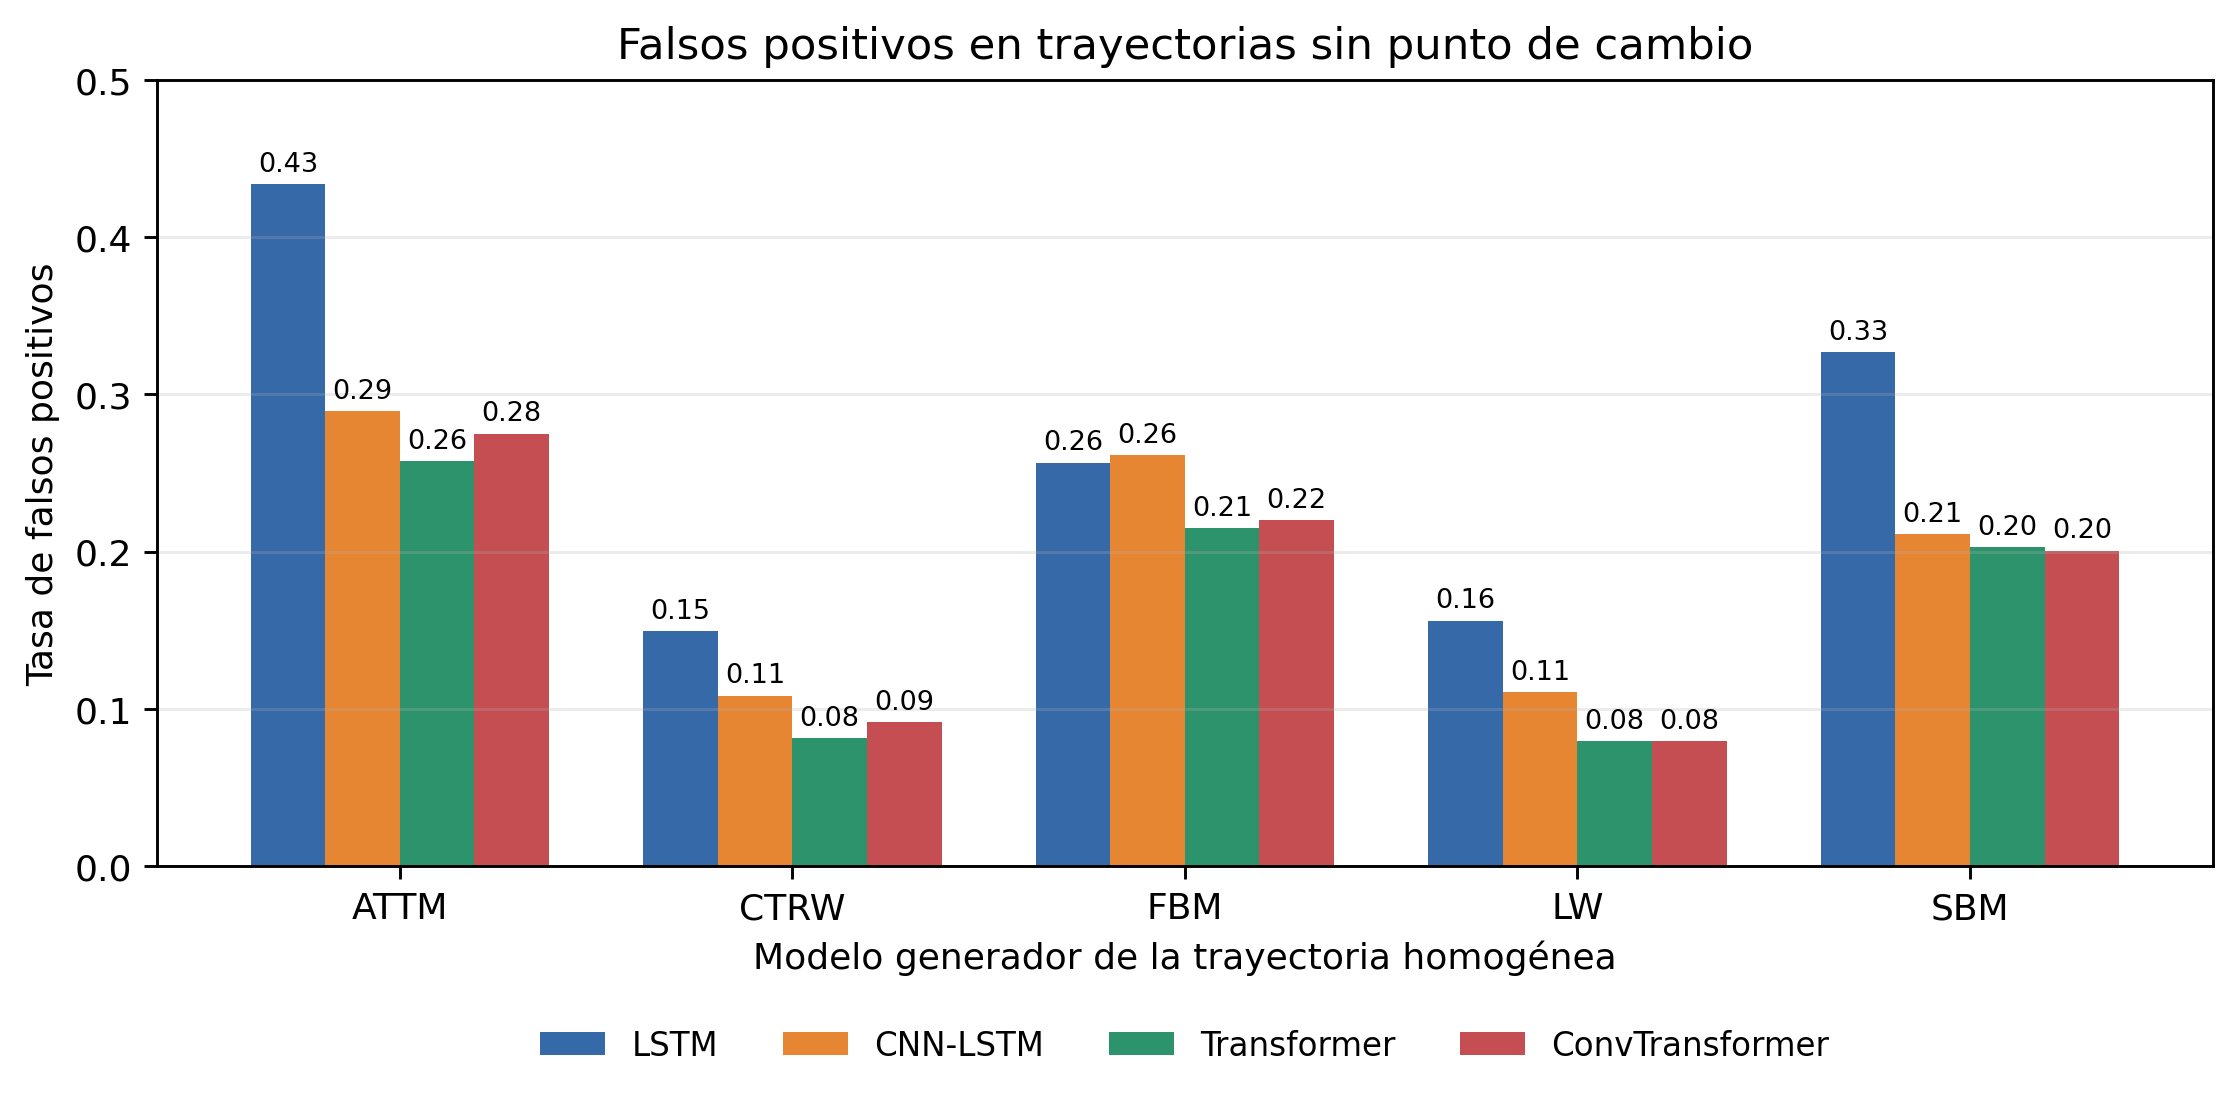
\includegraphics[width=\textwidth]{figures/revised/fpr_sin_cambio_comparacion.png}
\caption{Comparación de falsas alarmas con una escala común. Los valores proceden del conjunto de prueba del Protocolo B.}
\label{fig:fpr-model}
\end{figure}

ATTM es el negativo más difícil para las cuatro arquitecturas. La explicación física es compatible con la renovación interna de la difusividad: el proceso contiene cambios locales aun cuando no se ha concatenado otro modelo. SBM ocupa el segundo grupo de dificultad para LSTM y mantiene FPR cercanas a 0.20 en las redes restantes. Su no estacionariedad gradual puede producir diferencias entre regiones tempranas y tardías. FBM también genera falsas alarmas apreciables; aquí la fuente no es una varianza determinista, sino la correlación de los incrementos.

CTRW y LW presentan las menores FPR. Este resultado no implica que sean universalmente fáciles. Con la longitud, el ruido y la normalización utilizados, sus patrones parecen más distinguibles de una frontera entre modelos. Cambiar el rango de $\alpha$ o la duración podría alterar el orden.

La FPR global es 0.26445 para LSTM, 0.19602 para CNN--LSTM, 0.16721 para Transformer y 0.17324 para ConvTransformer. Transformer produce menos falsas alarmas, pero esta propiedad debe contrastarse con su sensibilidad ante trayectorias positivas. Un sistema puede reducir FPR simplemente adoptando decisiones conservadoras.

\section{Resultados en trayectorias con punto de cambio}
\label{sec:change-results}

\subsection{Detección binaria}

\begin{table}[htbp]
\centering
\footnotesize
\begin{tabular}{lccccccc}
\toprule
\textbf{Arquitectura} & $\boldsymbol\eta$ & \textbf{Acc.} & \textbf{Prec.} & \textbf{Recall} & \textbf{F1} & \textbf{FPR} & \textbf{FNR} \\
\midrule
LSTM & 0.35 & 0.7328 & 0.7341 & 0.7300 & 0.7320 & 0.2645 & 0.2700 \\
CNN--LSTM & 0.25 & 0.7891 & 0.7980 & 0.7743 & 0.7860 & 0.1960 & 0.2257 \\
Transformer & 0.30 & 0.7712 & 0.8093 & 0.7095 & 0.7561 & 0.1672 & 0.2905 \\
ConvTransformer & 0.30 & 0.8037 & 0.8184 & 0.7806 & 0.7990 & 0.1732 & 0.2194 \\
\bottomrule
\end{tabular}
\caption{Métricas globales de detección en el Protocolo B.}
\label{tab:global-detection}
\end{table}

\begin{figure}[htbp]
\centering
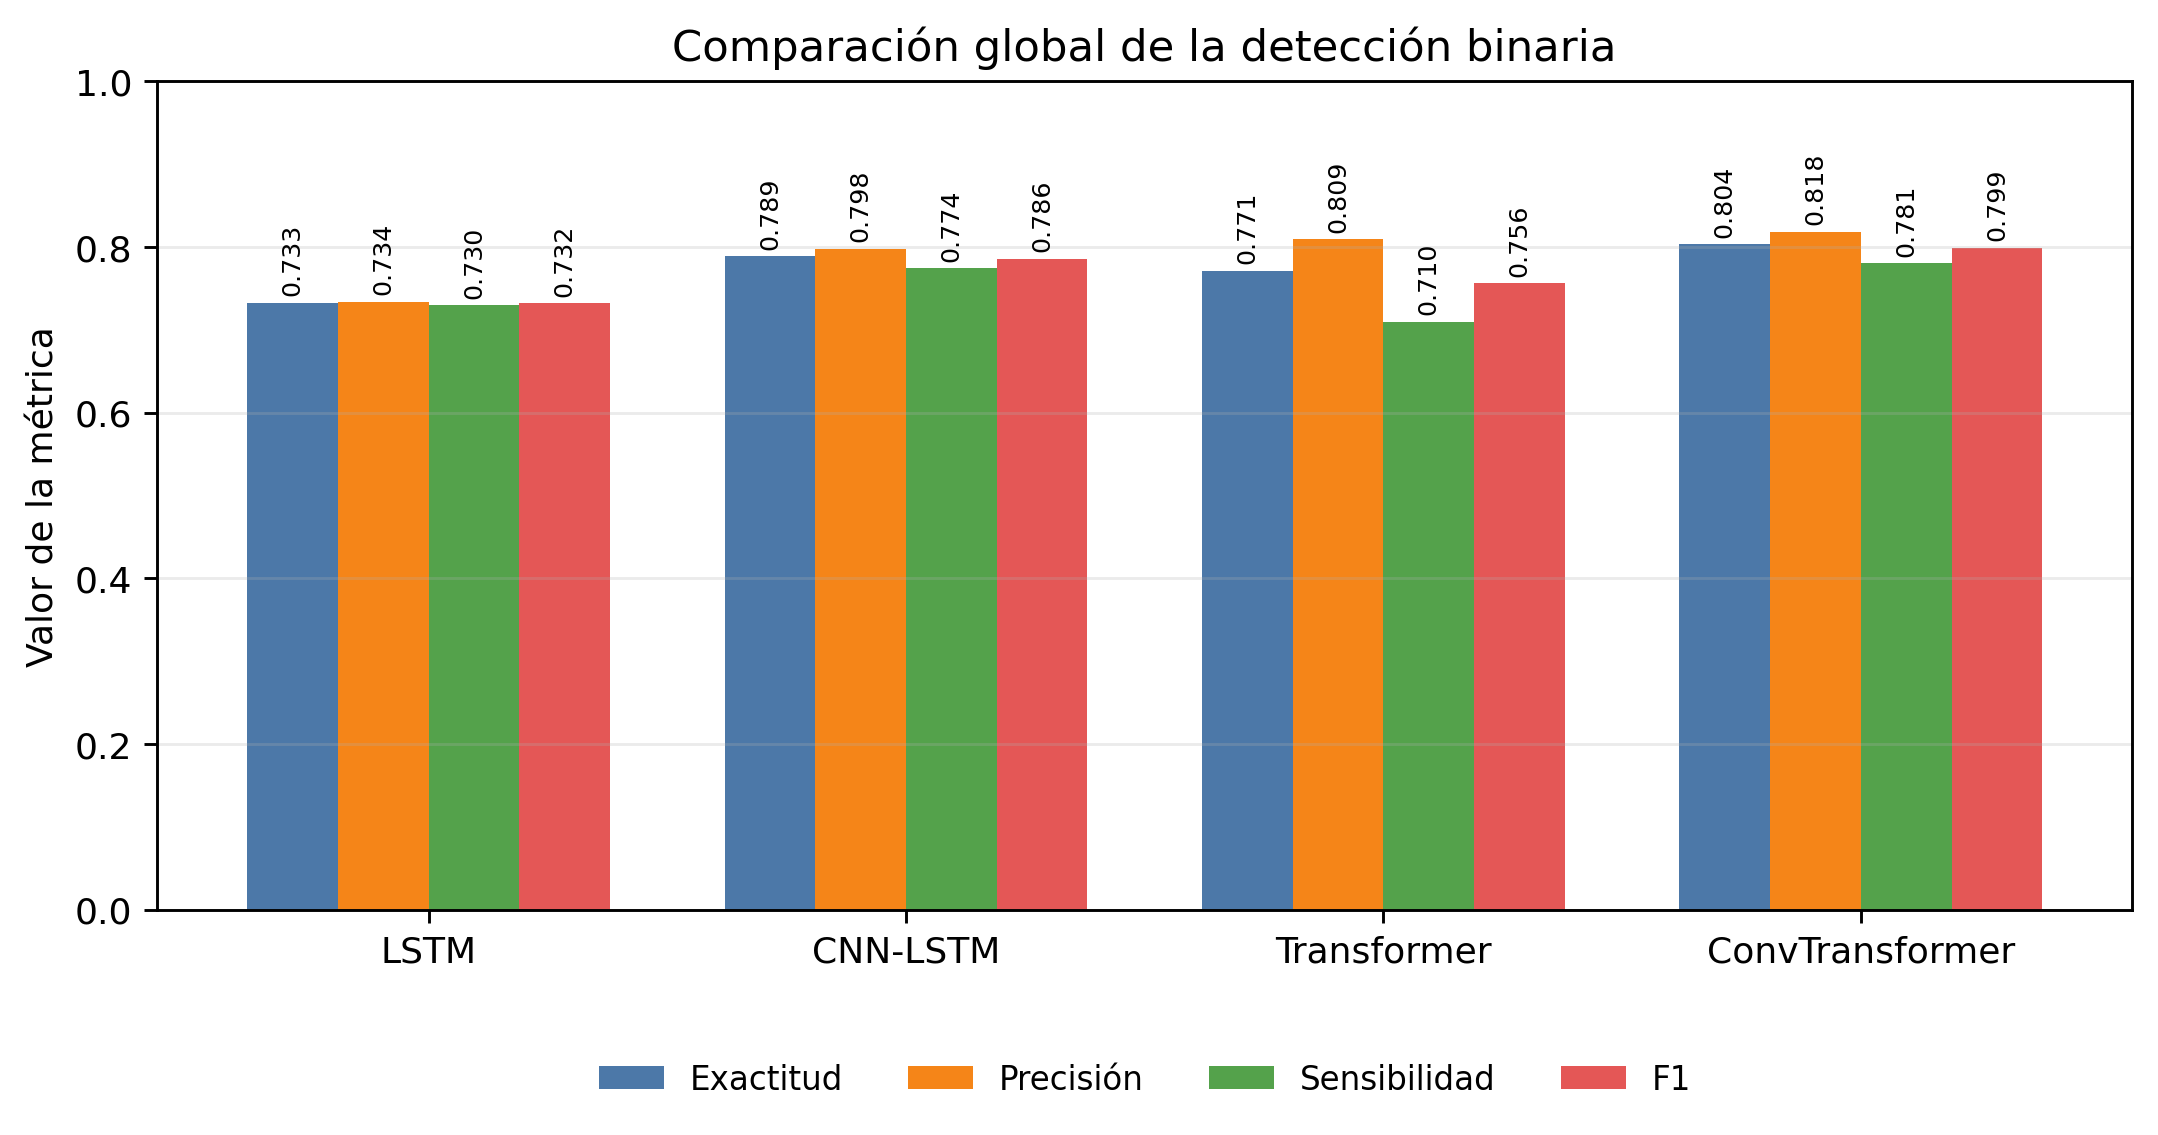
\includegraphics[width=\textwidth]{figures/revised/metricas_globales_deteccion.png}
\caption{Métricas globales de detección en escala $[0,1]$.}
\label{fig:global-detection}
\end{figure}

ConvTransformer alcanza el F1 más alto (0.7990) y la mayor sensibilidad (0.7806). CNN--LSTM queda próxima. Transformer obtiene la precisión más alta después de ConvTransformer y la FPR más baja, pero omite el 29.05\% de los cambios. Este patrón confirma un detector más conservador. LSTM ofrece el comportamiento menos favorable en las métricas agregadas.

Las diferencias no pueden atribuirse solo a la arquitectura. Tres modelos penalizan la clase negativa con peso 1.8, mientras LSTM utiliza BCE no ponderada; además, los umbrales se seleccionaron con restricciones distintas. Los valores describen sistemas completos --arquitectura, pérdida, selección y umbral--, no bloques neuronales aislados.

\subsection{Localización temporal}

\begin{table}[htbp]
\centering
\small
\begin{tabular}{lrrrr}
\toprule
\textbf{Arquitectura} & \textbf{MAE all} & \textbf{RMSE all} & \textbf{MAE TP} & \textbf{RMSE TP} \\
\midrule
LSTM & 12.7331 & 16.3504 & 11.4039 & 15.0504 \\
CNN--LSTM & 7.6645 & 11.9183 & 5.9136 & 9.9519 \\
Transformer & 8.7414 & 12.5307 & 6.6877 & 10.4040 \\
ConvTransformer & 7.5370 & 11.5706 & 5.7797 & 9.6215 \\
\bottomrule
\end{tabular}
\caption{Errores de localización en muestras temporales. \emph{All} incluye toda trayectoria con cambio real; TP se restringe a cambios detectados.}
\label{tab:global-localization}
\end{table}

\begin{figure}[htbp]
\centering
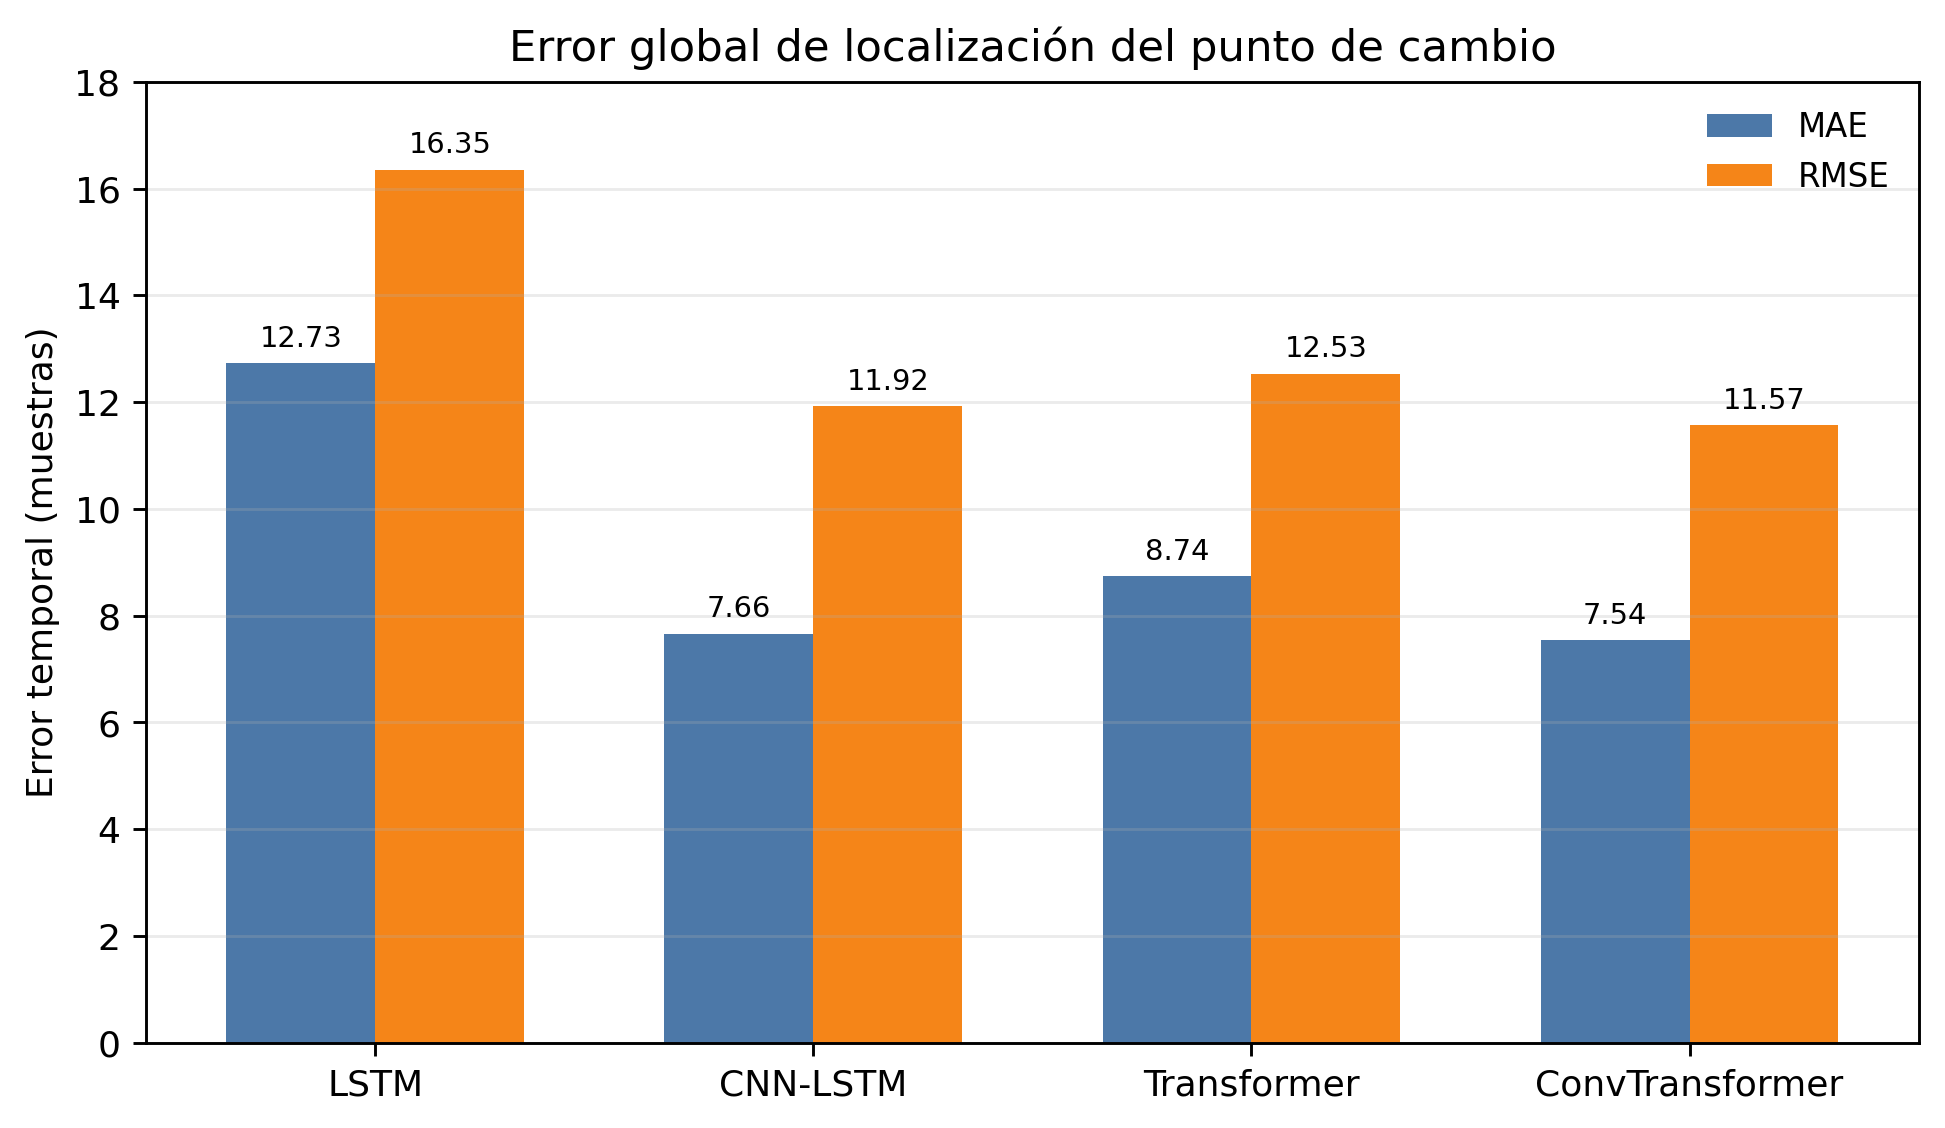
\includegraphics[width=0.95\textwidth]{figures/revised/errores_globales_localizacion.png}
\caption{MAE y RMSE globales de localización sobre todas las trayectorias con cambio.}
\label{fig:global-localization}
\end{figure}

Las dos arquitecturas con convoluciones obtienen los menores errores. ConvTransformer presenta MAE 7.537 y CNN--LSTM 7.664; la diferencia de 0.127 muestras es demasiado pequeña para interpretarla sin repeticiones entre semillas. El resultado sólido es que ambas configuraciones superan ampliamente a LSTM en esta ejecución. Transformer queda en una posición intermedia.

La diferencia entre métricas \emph{all} y TP muestra que los ejemplos omitidos por la cabeza binaria también suelen ser difíciles de localizar. Reportar solo MAE en verdaderos positivos produciría una estimación optimista del sistema completo.

El Apéndice~\ref{app:qualitative-examples} muestra cuatro predicciones de ConvTransformer-v2 para complementar esta lectura cuantitativa sin convertir una selección visual en evidencia de rendimiento.

\subsection{Estabilidad de ConvTransformer-v2 frente a la inicialización}
\label{sec:convtransformer-multiseed}

La ejecución principal de ConvTransformer-v2 se complementó con cinco entrenamientos correspondientes a las semillas 1, 2, 3, 42 y 123. Para que la información de entrenamiento fuera idéntica entre repeticiones, se fijó mediante una semilla independiente el mismo subconjunto equilibrado de 10\,000 trayectorias. Cada modelo utilizó hasta 20 épocas, lote 1024, la validación completa de 20\,000 trayectorias y el test completo de 200\,000. El umbral se seleccionó por separado en validación para cada semilla. Por tanto, el experimento mide la sensibilidad a la inicialización bajo un presupuesto reducido y no reproduce exactamente el entrenamiento principal.

\begin{table}[htbp]
\centering
\small
\begin{tabular}{lc}
\toprule
\textbf{Métrica} & \textbf{Media $\boldsymbol{\pm}$ desviación estándar} \\
\midrule
Accuracy & $0.5627 \pm 0.0869$ \\
Precision & $0.5780 \pm 0.1070$ \\
Recall & $0.8227 \pm 0.2453$ \\
F1-score & $0.6469 \pm 0.0363$ \\
FPR & $0.6974 \pm 0.4144$ \\
FNR & $0.1773 \pm 0.2453$ \\
MAE \emph{all} & $14.4826 \pm 1.1010$ \\
RMSE \emph{all} & $17.0397 \pm 0.8186$ \\
nMAE \emph{all} & $0.1448 \pm 0.0110$ \\
nRMSE \emph{all} & $0.1704 \pm 0.0082$ \\
MAE TP & $14.0182 \pm 1.7433$ \\
RMSE TP & $16.6425 \pm 1.3707$ \\
\bottomrule
\end{tabular}
\caption{Resultados de ConvTransformer-v2 con cinco semillas bajo el protocolo reducido de entrenamiento. La normalización de nMAE y nRMSE emplea $L=100$.}
\label{tab:convtransformer-multiseed}
\end{table}

La dispersión no se limita a pequeñas fluctuaciones numéricas. Las semillas 2, 3 y 123 convergieron hacia clasificadores que marcaron casi todas las trayectorias como positivas, con FPR próximas a 1. Las semillas 1 y 42 produjeron soluciones no degeneradas, con FPR de 0.2321 y 0.2550, respectivamente. En un test equilibrado, predecir siempre la clase positiva genera recall 1 y F1 cercano a 0.667; por ello, el F1 medio y su desviación relativamente pequeña ocultan un comportamiento inaceptable que sí revelan la FPR y las matrices de confusión.

El resultado principal de ConvTransformer-v2, entrenado con el protocolo completo, alcanzó F1 0.7990 y FPR 0.1732. No debe compararse directamente con la media del Cuadro~\ref{tab:convtransformer-multiseed}, porque cambian el tamaño de entrenamiento, el lote y el límite de épocas. La conclusión válida del experimento multisemilla es más acotada: con solo 10\,000 trayectorias, la optimización de ConvTransformer-v2 es sensible a la inicialización y puede converger hacia soluciones degeneradas. Una estimación confirmatoria de la variabilidad del modelo principal requeriría repetir el entrenamiento completo con las mismas cinco semillas.

\subsection{Comparación con la baseline PELT}
\label{sec:pelt-results}

\begin{table}[htbp]
\centering
\footnotesize
\begin{tabular}{lrrrrrrrr}
\toprule
\textbf{Método} & \textbf{Acc.} & \textbf{Prec.} & \textbf{Recall} & \textbf{F1} &
\textbf{FPR} & \textbf{FNR} & \textbf{MAE TP} & \textbf{RMSE TP} \\
\midrule
ConvTransformer-v2 & 0.8037 & 0.8184 & 0.7806 & 0.7990 & 0.1732 & 0.2194 & 5.7797 & 9.6215 \\
PELT & 0.5341 & 0.5346 & 0.5259 & 0.5302 & 0.4578 & 0.4741 & 16.3166 & 22.3348 \\
\bottomrule
\end{tabular}
\caption{Comparación sobre el test completo de $L=100$. ConvTransformer-v2 corresponde a la ejecución principal; PELT es una baseline sin entrenamiento supervisado. Los errores temporales se restringen a verdaderos positivos.}
\label{tab:convtransformer-pelt}
\end{table}

PELT obtuvo F1 0.5302, FPR 0.4578 y FNR 0.4741. En consecuencia, la segmentación penalizada basada en energía y amplitud absoluta apenas separa las trayectorias homogéneas de las que contienen una transición. Cuando el cambio fue detectado, su MAE fue 16.32 muestras, frente a 5.78 para ConvTransformer-v2. Al penalizar con 100 muestras los cambios omitidos, PELT alcanzó MAE global 55.99 y RMSE global 70.73; estos dos últimos valores integran el fallo de detección y no son directamente equivalentes a la salida temporal \emph{all} de la red.

La comparación muestra que esta configuración simple de PELT no captura suficientemente las modificaciones de correlación, intermitencia y no estacionariedad presentes en los cinco generadores. No demuestra que cualquier método clásico sea inferior ni que ConvTransformer supere a los participantes de AnDi. Una baseline clásica más amplia debería estudiar otros costes y características locales, como autocorrelación, inmovilidad o estimaciones locales del exponente.

\subsection{Transiciones ordenadas}

\begin{figure}[htbp]
\centering
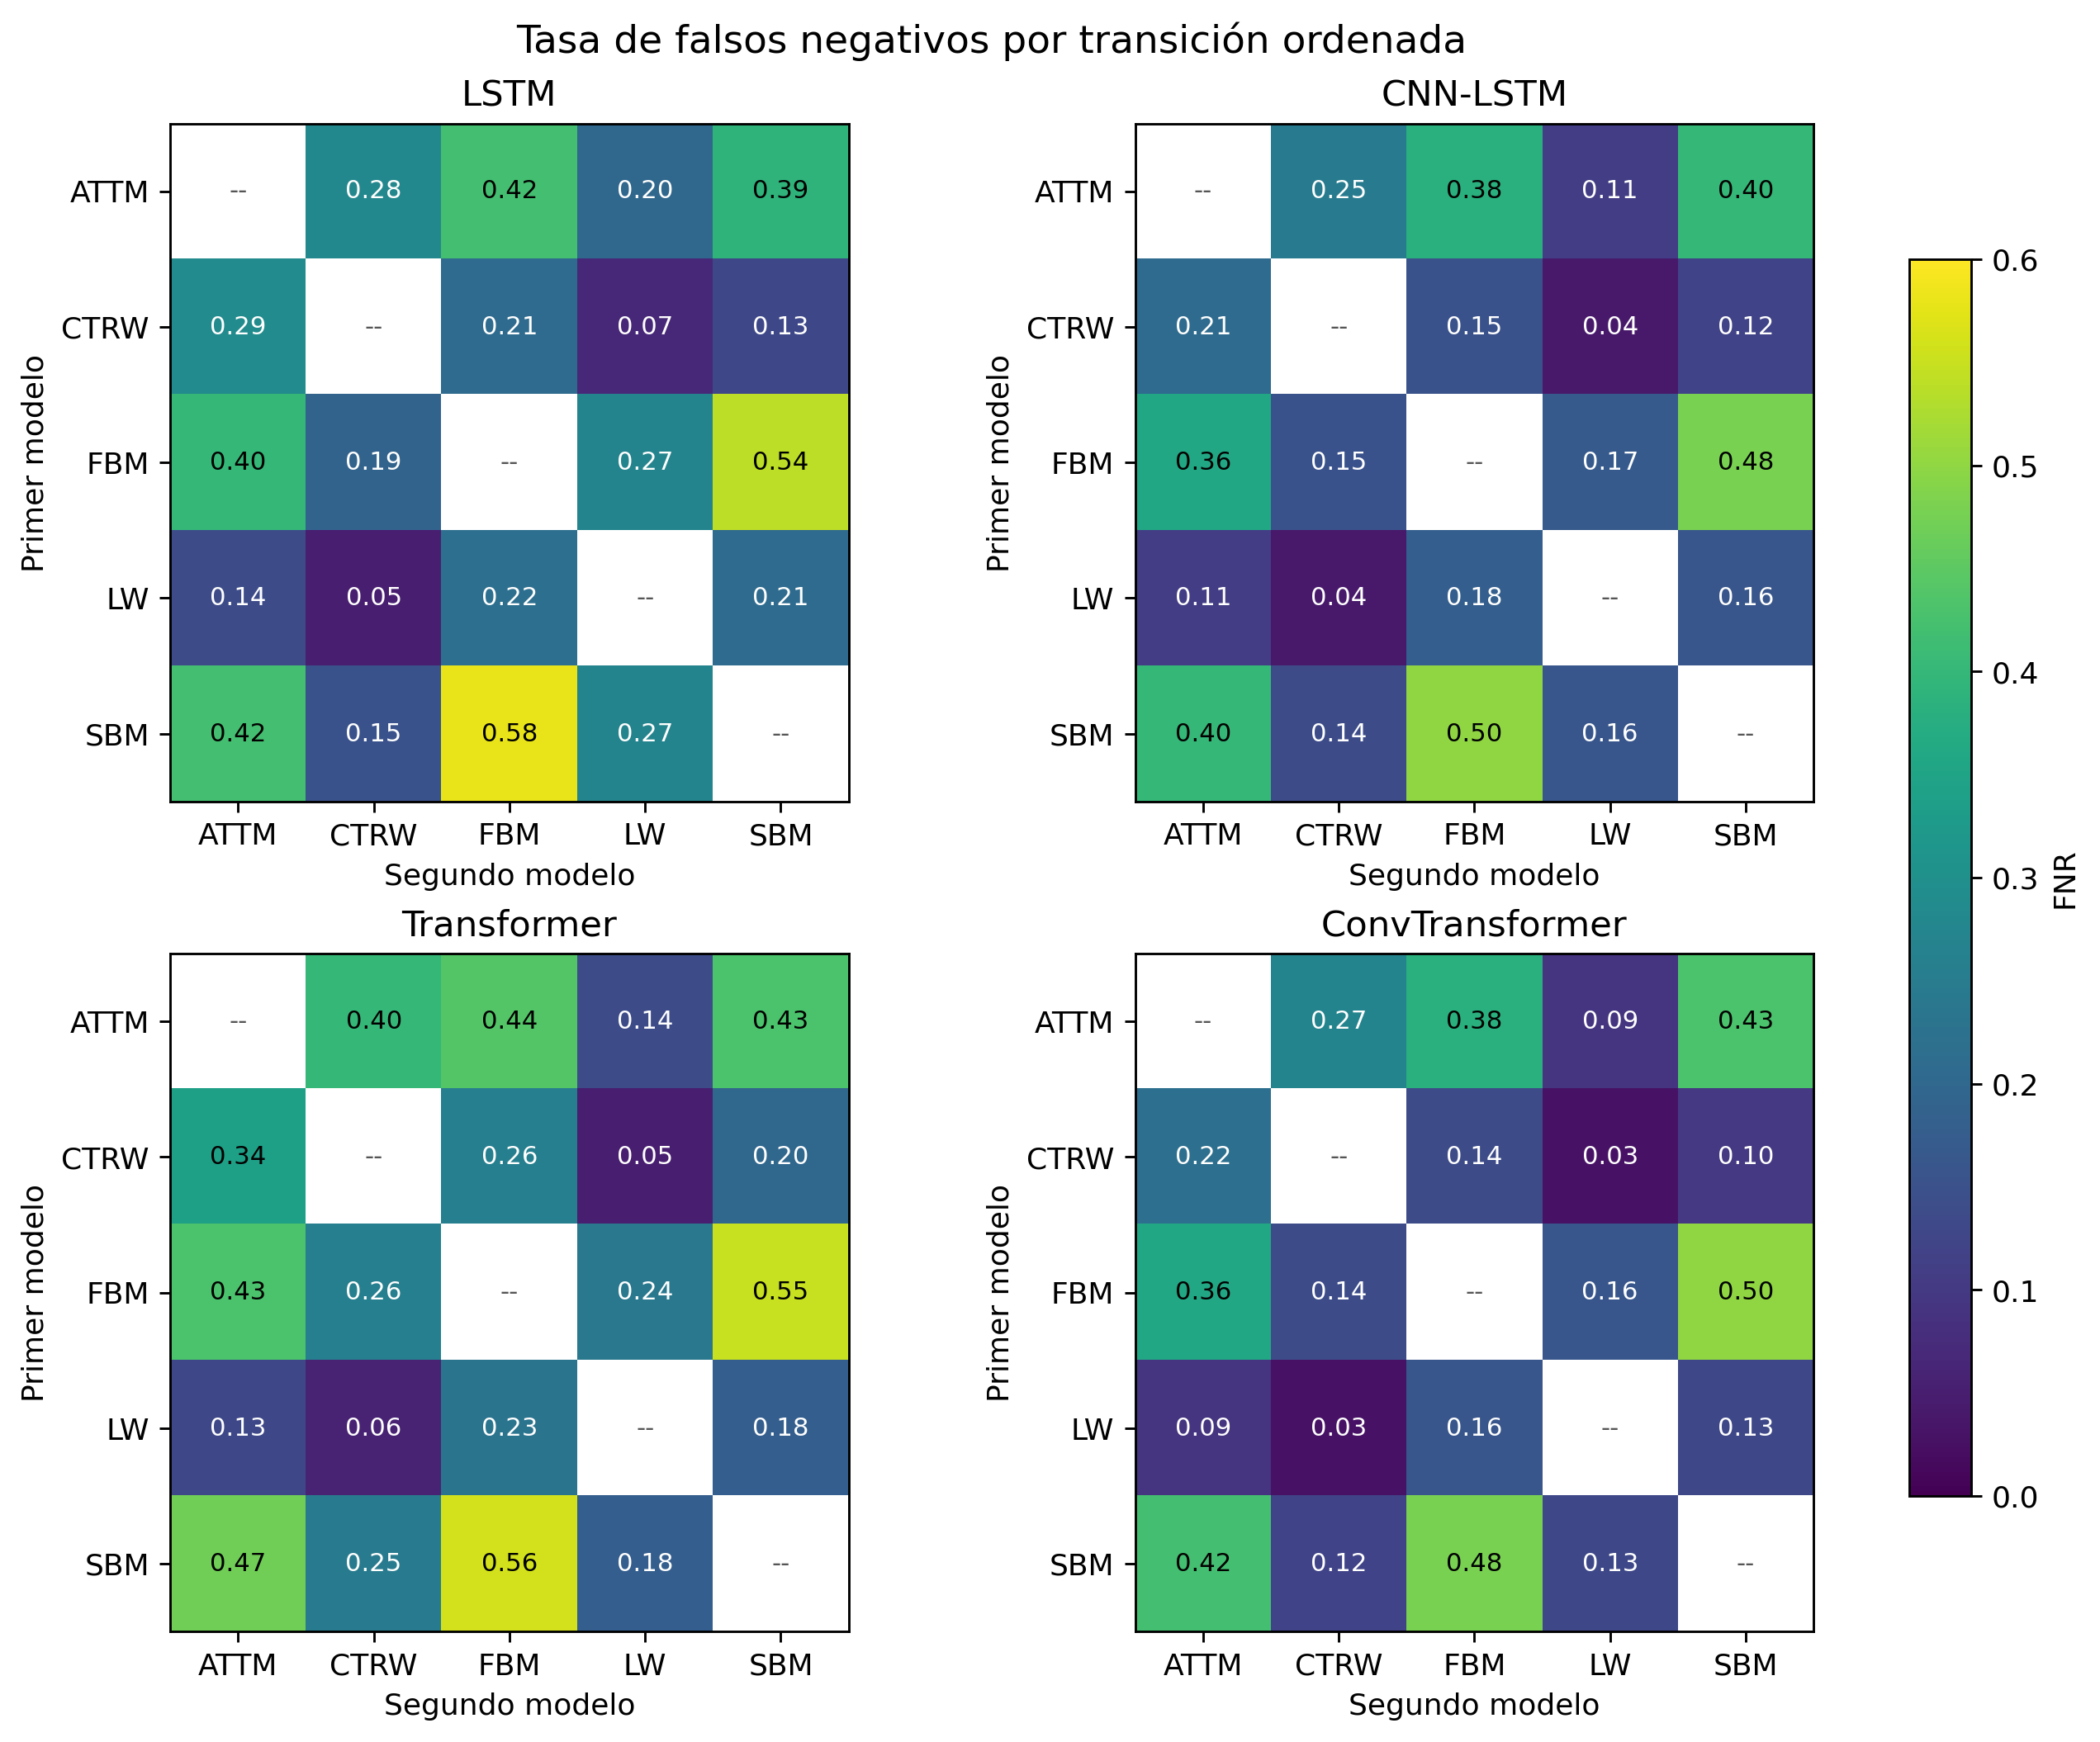
\includegraphics[width=0.96\textwidth]{figures/revised/fnr_transiciones.png}
\caption{FNR por transición ordenada para $L=100$. En cada matriz, las filas indican el modelo del primer segmento y las columnas el del segundo; la escala común permite reconocer valores altos en FBM$\to$SBM y SBM$\to$FBM y valores bajos en CTRW$\leftrightarrow$LW.}
\label{fig:fnr-transition}
\end{figure}

La Figura~\ref{fig:fnr-transition} revela una estructura común. Las transiciones con FBM o SBM como segundo modelo concentran FNR elevadas cuando el primer régimen también presenta correlación, heterogeneidad o no estacionariedad. Por ejemplo, FBM$\to$SBM y SBM$\to$FBM se encuentran entre los pares más difíciles. En cambio, CTRW$\leftrightarrow$LW genera FNR reducidas. La asimetría confirma que invertir el orden cambia la evidencia disponible: los segmentos ocupan posiciones temporales distintas y SBM no posee incrementos estacionarios.

\begin{figure}[htbp]
\centering
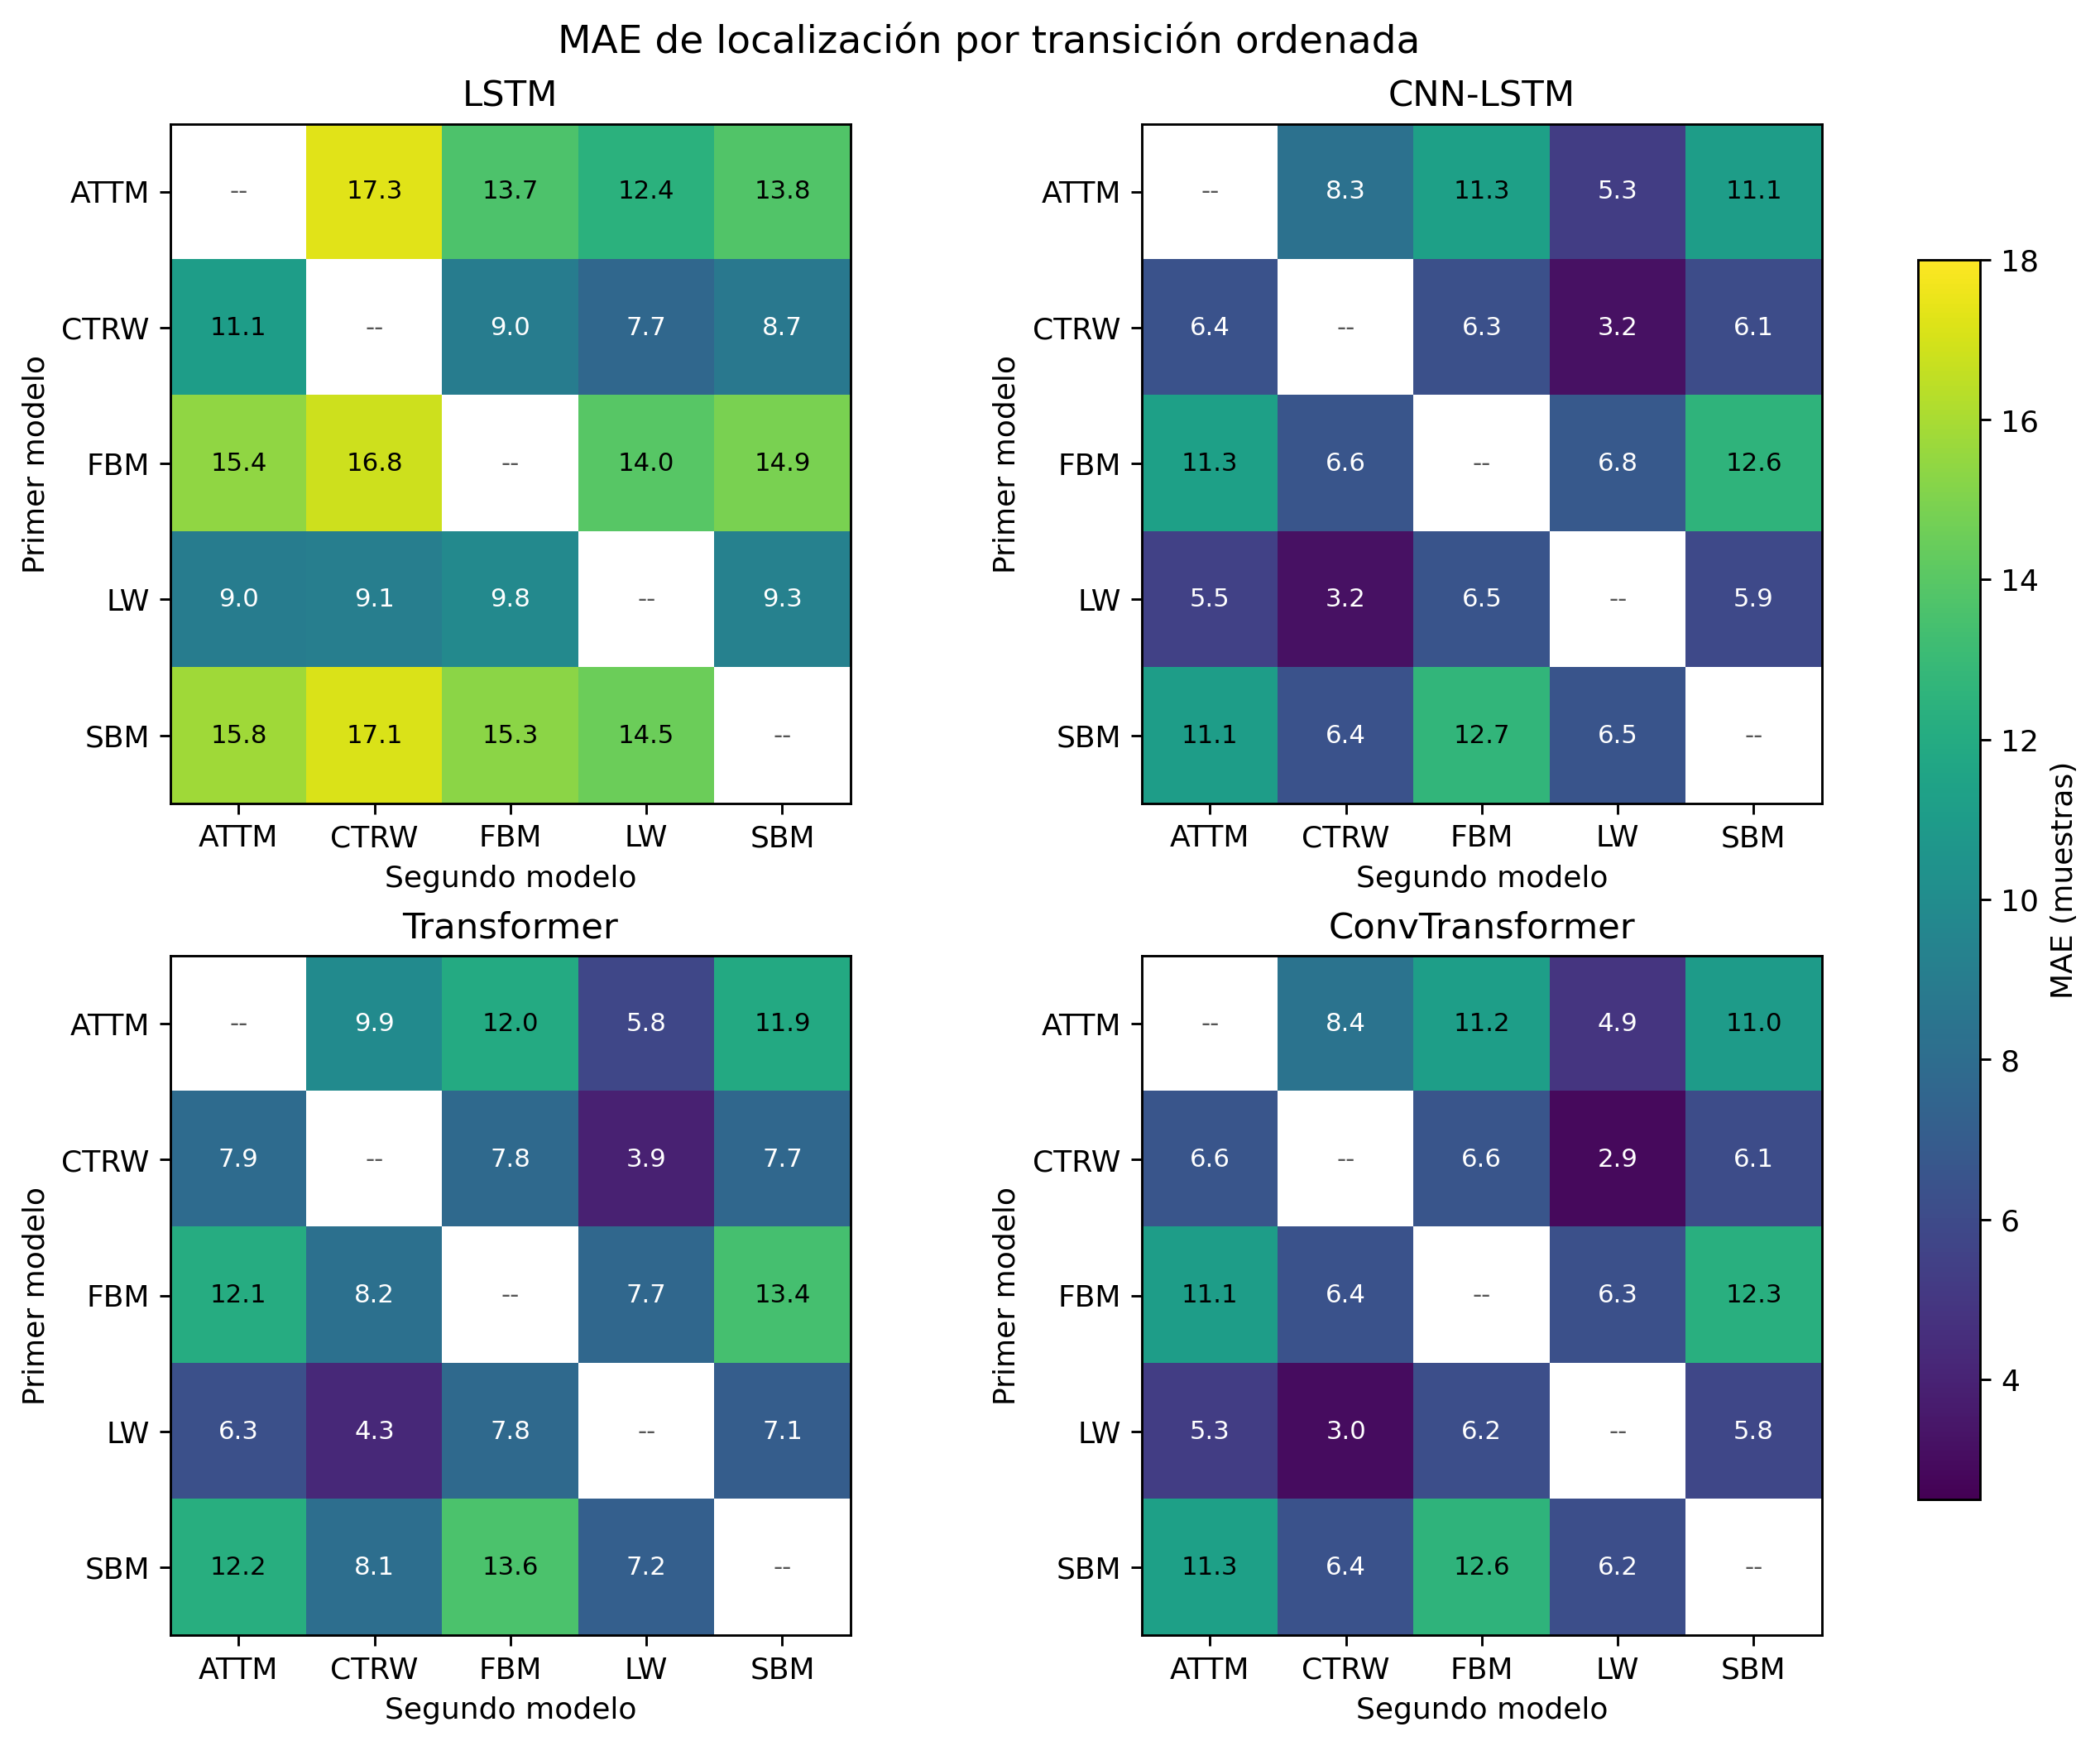
\includegraphics[width=0.96\textwidth]{figures/revised/mae_transiciones.png}
\caption{MAE de localización sobre todas las trayectorias positivas, por transición ordenada ($L=100$). Filas: primer modelo; columnas: segundo modelo. LSTM concentra errores altos cuando ATTM, FBM o SBM ocupan el primer segmento; las arquitecturas convolucionales reducen especialmente los errores asociados a LW.}
\label{fig:mae-transition}
\end{figure}

\begin{figure}[htbp]
\centering
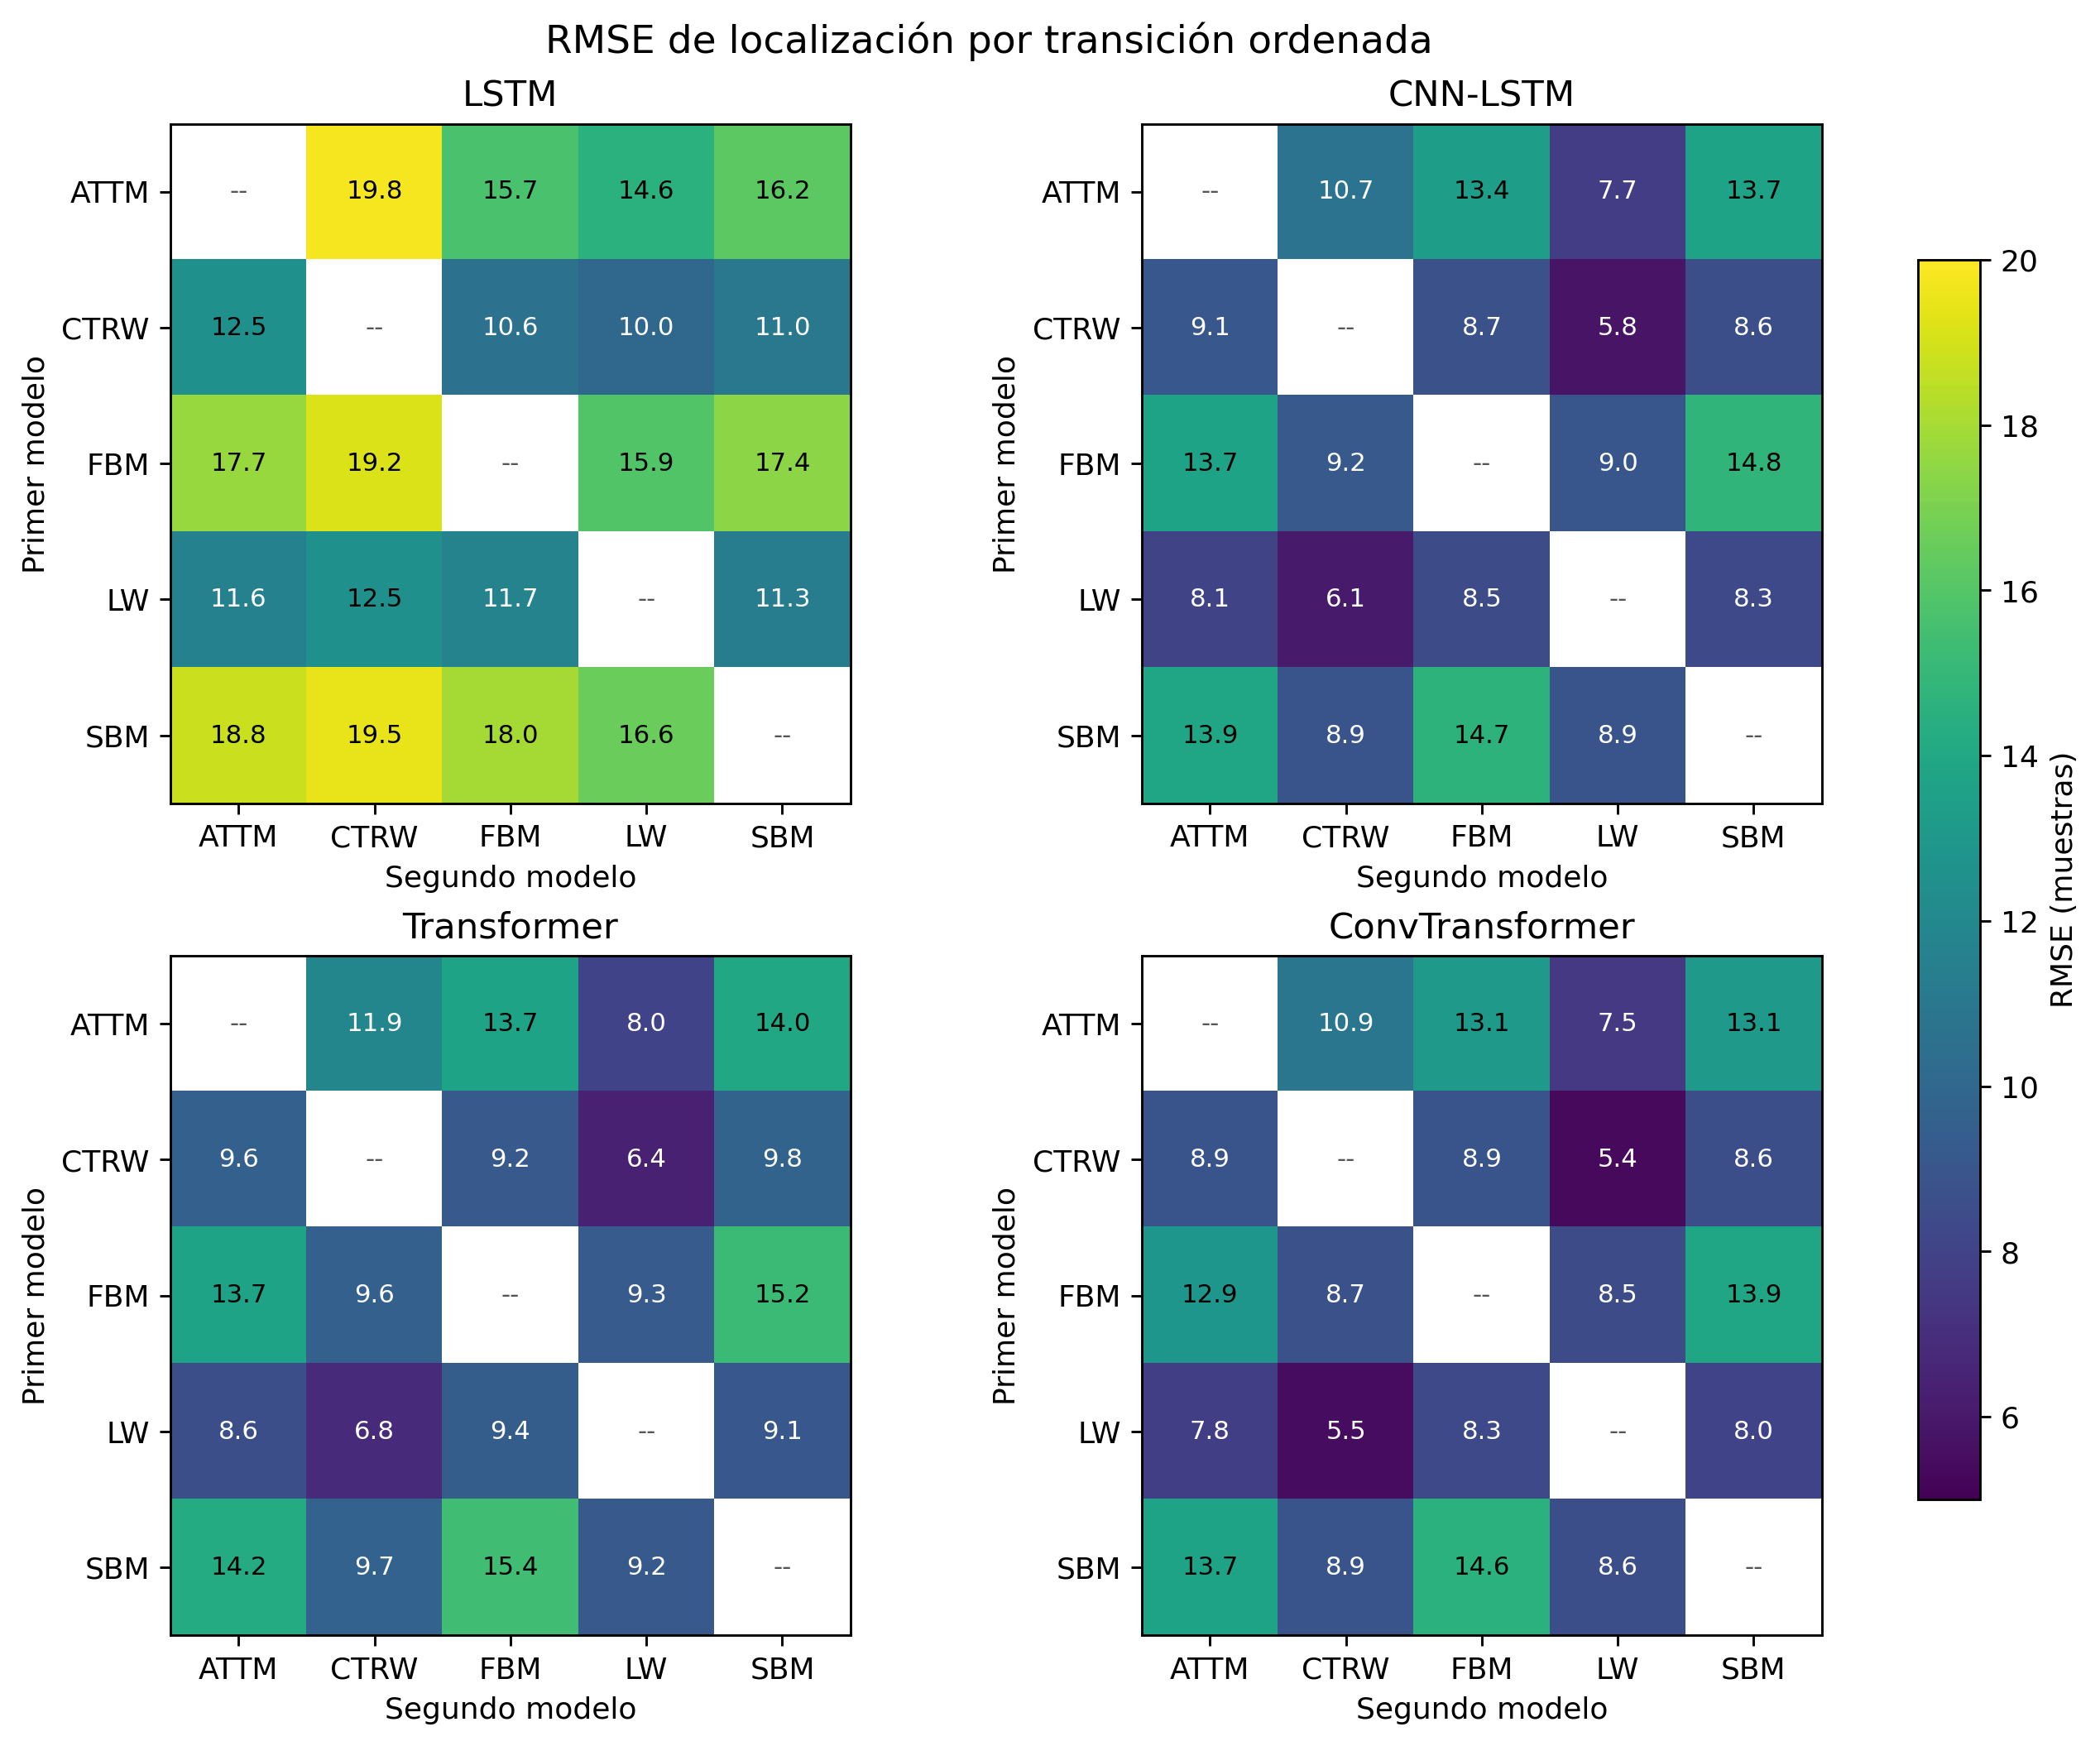
\includegraphics[width=0.96\textwidth]{figures/revised/rmse_transiciones.png}
\caption{RMSE de localización sobre todas las trayectorias positivas, por transición ordenada ($L=100$), con filas = primer modelo y columnas = segundo modelo. El mayor peso de errores extremos mantiene como difíciles varias transiciones con FBM o SBM.}
\label{fig:rmse-transition}
\end{figure}

MAE y RMSE mantienen el mismo patrón general, aunque RMSE amplifica los fallos extremos. LSTM presenta errores altos en casi todas las transiciones que empiezan en ATTM, FBM o SBM. CNN--LSTM y ConvTransformer reducen especialmente el error cuando LW participa en la frontera. El contraste entre CTRW y LW parece contener rasgos locales que las convoluciones explotan con eficacia.

No debe concluirse que una pareja es intrínsecamente fácil o difícil. Los rangos de $\alpha$ no coinciden entre modelos y se muestrean independientemente; por tanto, las matrices combinan mecanismo, exponente, ruido y posición.

\subsection{ConvTransformer a dos longitudes}
\label{sec:convtransformer-lengths}

La comparación anterior identifica ConvTransformer como la mejor configuración observada para $L=100$. A partir de esa selección se fija la familia arquitectónica y se repite el protocolo binario con $L=200$. En ambos casos se conservan el extractor convolucional, los dos bloques residuales dilatados, tres bloques Transformer, cinco modelos generadores y 20 transiciones ordenadas. La frontera se restringe al mismo intervalo relativo, 20--80\% de la trayectoria. Cada celda de las Figuras~\ref{fig:convtransformer-l100} y \ref{fig:convtransformer-l200} resume 5000 trayectorias positivas de prueba; la fila indica el modelo del primer segmento y la columna, el del segundo.

Para comparar errores entre longitudes se utilizan
\begin{equation}
  \mathrm{nMAE}=\frac{\mathrm{MAE}_{\mathrm{all}}}{L},
  \qquad
  \mathrm{nRMSE}=\frac{\mathrm{RMSE}_{\mathrm{all}}}{L}.
  \label{eq:normalized-localization-errors}
\end{equation}
La normalización evita que un error de igual proporción temporal parezca peor solo por contener más muestras. El subíndice \emph{all} indica que se incluyen todas las trayectorias con cambio, también las que la cabeza binaria no detecta.

\begin{table}[htbp]
\centering
\scriptsize
\resizebox{\textwidth}{!}{%
\begin{tabular}{cccccccccccc}
\toprule
$\boldsymbol L$ & $\boldsymbol\eta$ & \textbf{Acc.} & \textbf{Prec.} & \textbf{Recall} & \textbf{F1} & \textbf{FPR} & \textbf{FNR} & \textbf{MAE} & \textbf{RMSE} & \textbf{nMAE} & \textbf{nRMSE} \\
\midrule
100 & 0.300 & 0.8037 & 0.8184 & 0.7806 & 0.7990 & 0.1732 & 0.2194 & 7.5370 & 11.5706 & 0.0754 & 0.1157 \\
200 & 0.475 & 0.8524 & 0.8944 & 0.7990 & 0.8440 & 0.0943 & 0.2010 & 9.3761 & 18.2741 & 0.0469 & 0.0914 \\
\bottomrule
\end{tabular}}
\caption{ConvTransformer en los conjuntos de prueba de longitudes 100 y 200. Los errores no normalizados se expresan en muestras.}
\label{tab:convtransformer-lengths}
\end{table}

\begin{figure}[htbp]
\centering
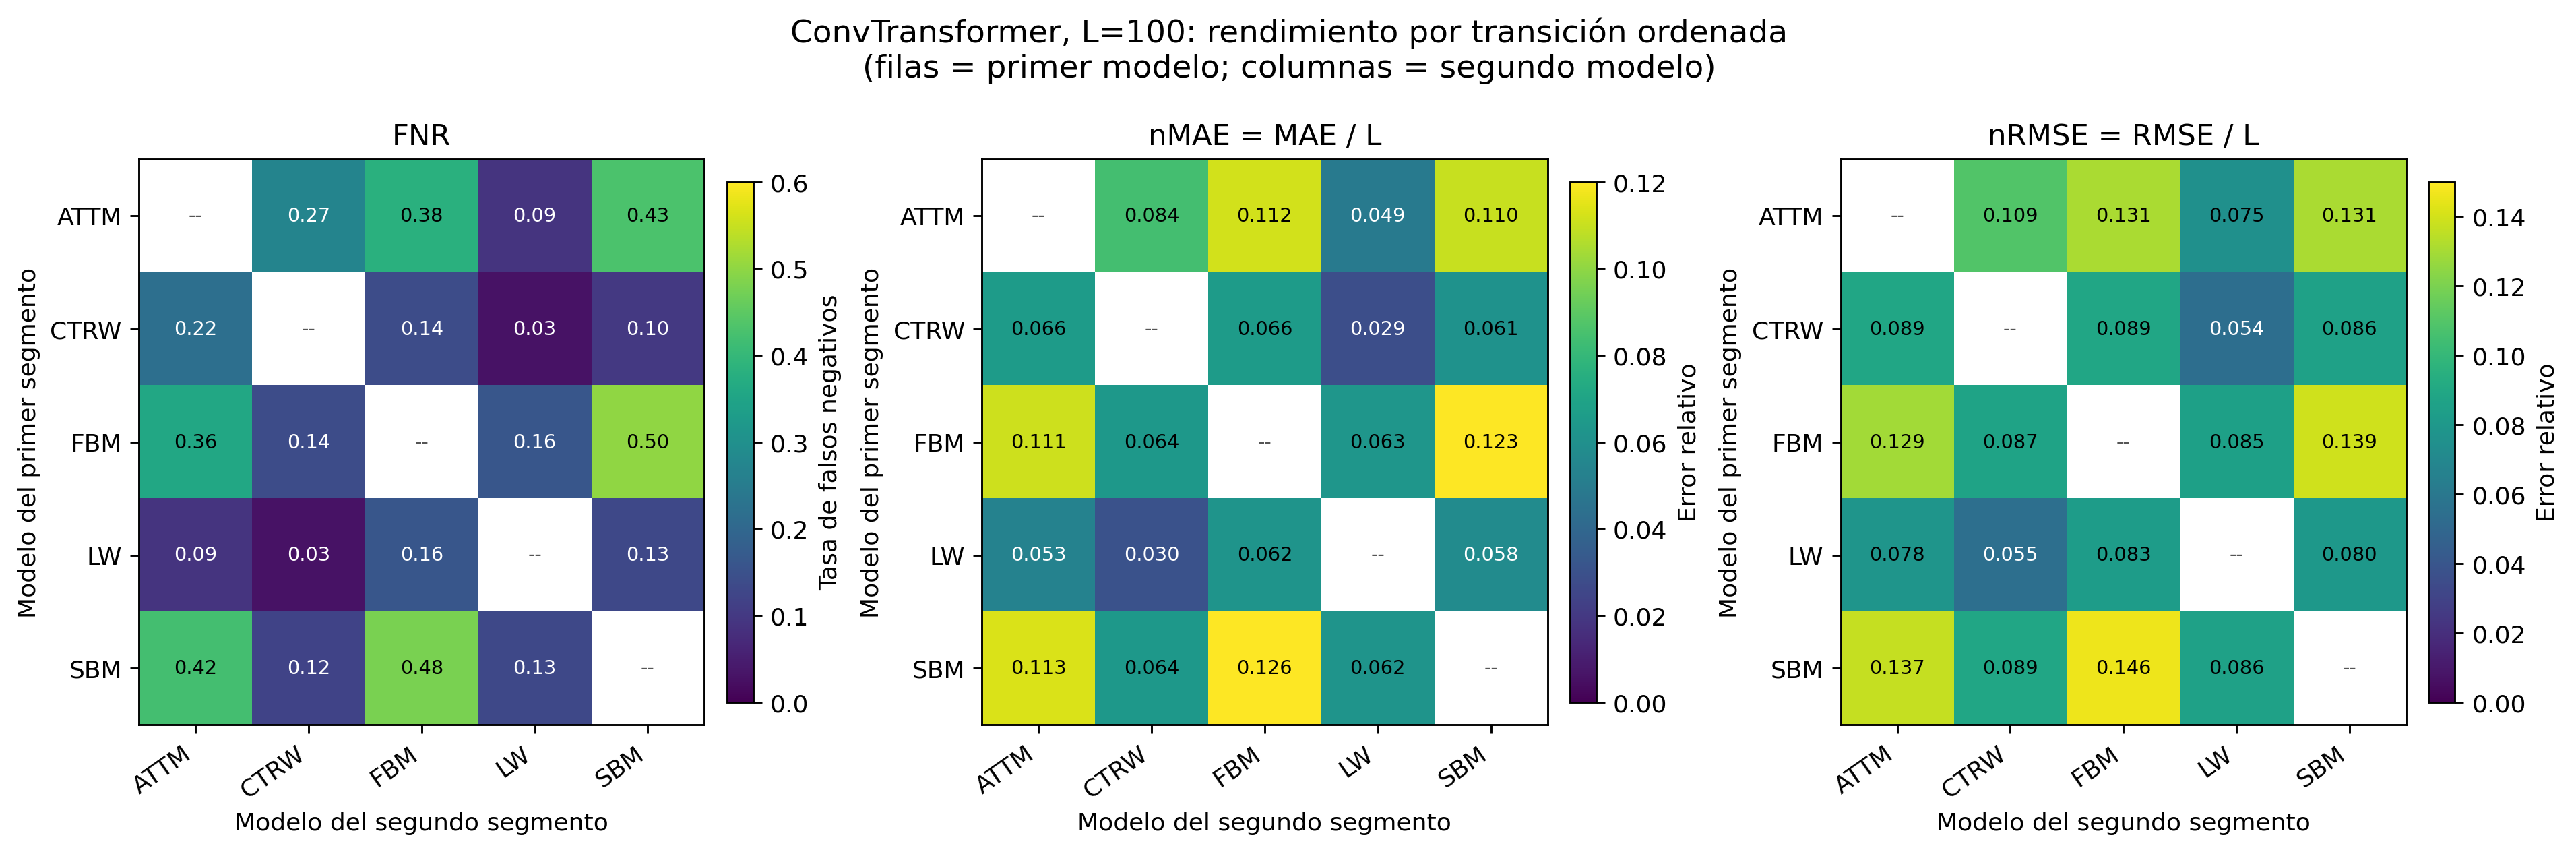
\includegraphics[width=\textwidth]{figures/revised/convtransformer_transiciones_L100.png}
\caption{ConvTransformer, $L=100$: FNR, nMAE y nRMSE por transición ordenada. Filas = primer modelo; columnas = segundo modelo. FBM$\to$SBM y SBM$\to$FBM destacan por FNR y error relativo elevados, mientras CTRW$\leftrightarrow$LW resulta favorable.}
\label{fig:convtransformer-l100}
\end{figure}

\begin{figure}[htbp]
\centering
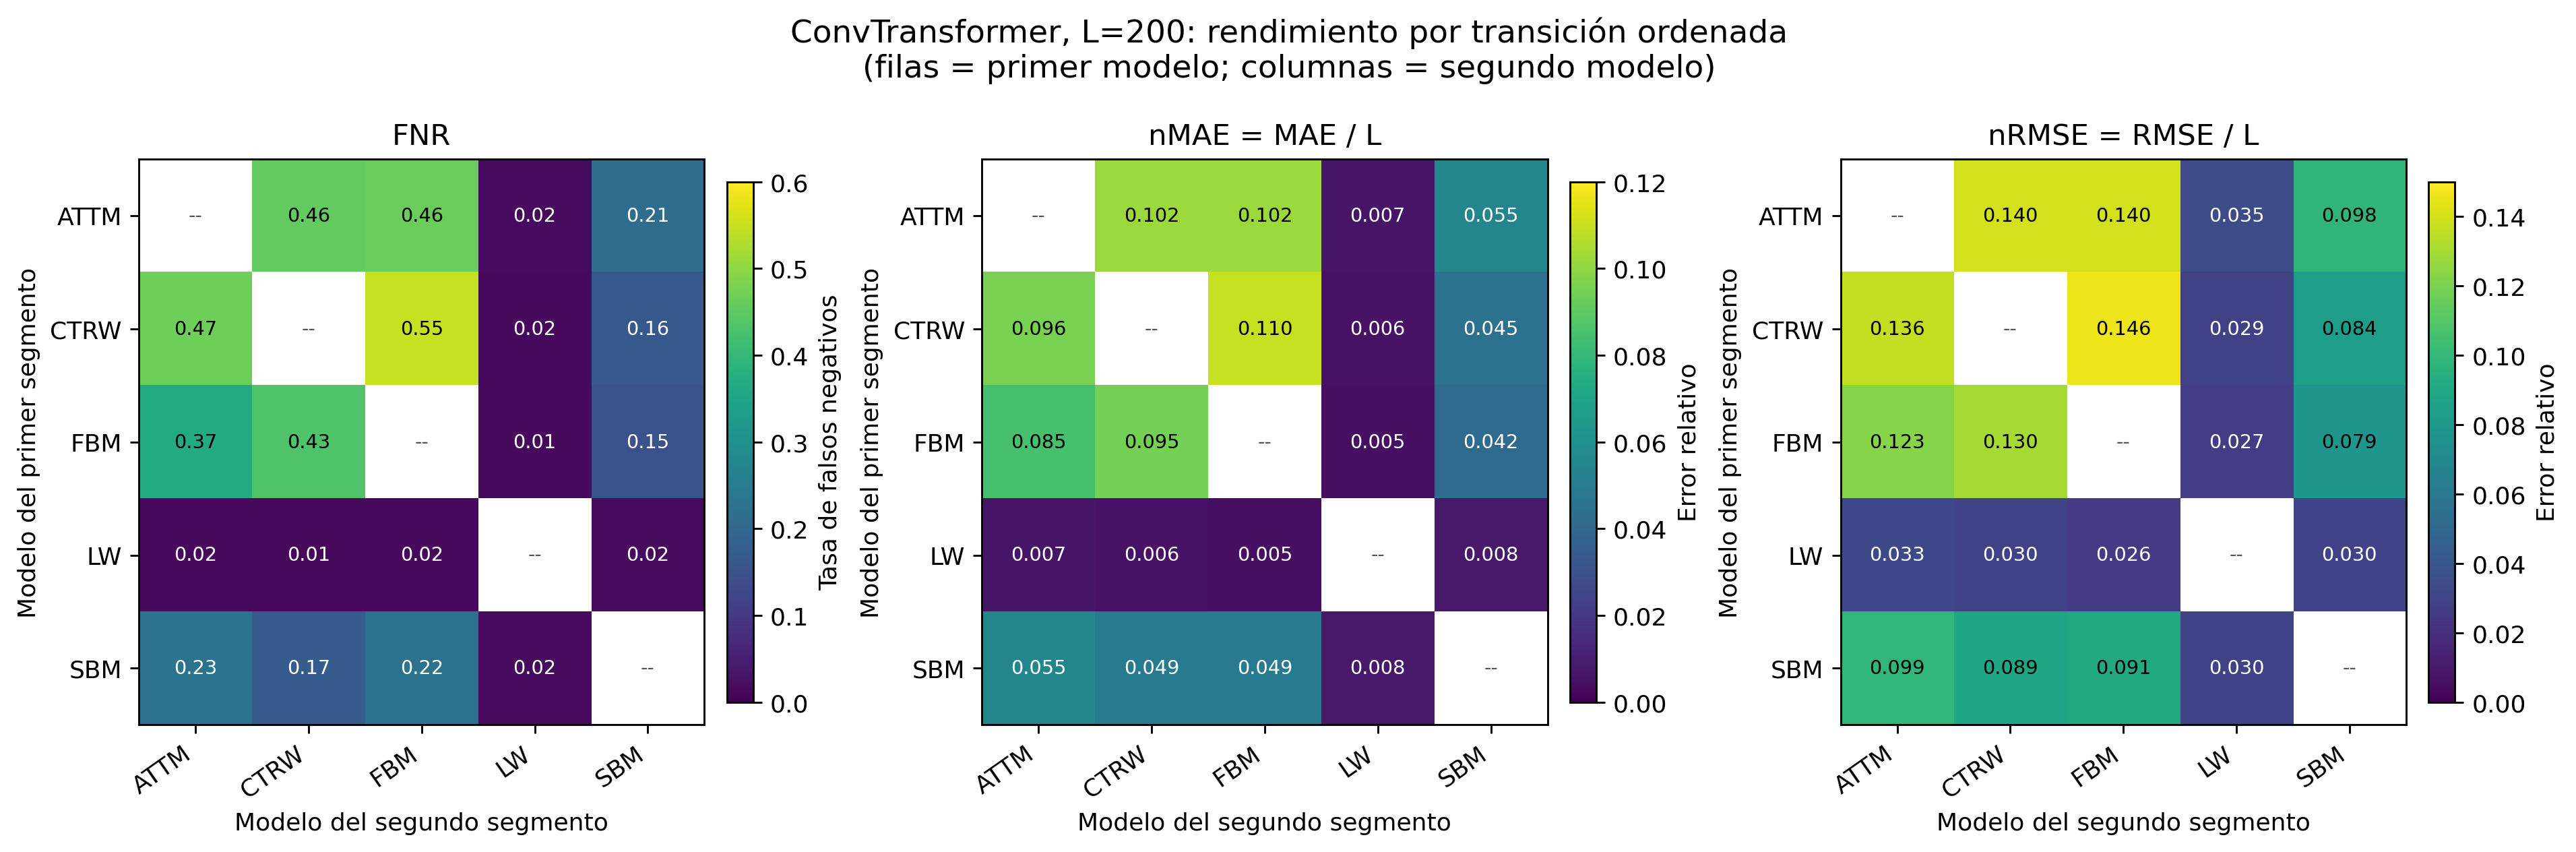
\includegraphics[width=\textwidth]{figures/revised/convtransformer_transiciones_L200.png}
\caption{ConvTransformer, $L=200$: FNR, nMAE y nRMSE de la ejecución global. Filas = primer modelo; columnas = segundo modelo. CTRW$\to$FBM es la transición más problemática; las parejas que incluyen LW presentan los valores más bajos.}
\label{fig:convtransformer-l200}
\end{figure}

La longitud adicional no beneficia por igual a todas las parejas. En $L=100$, las mayores FNR aparecen en FBM$\to$SBM (0.50), SBM$\to$FBM (0.48), ATTM$\to$SBM (0.43) y SBM$\to$ATTM (0.42). En $L=200$, el foco de dificultad se desplaza hacia CTRW$\to$FBM (0.55), CTRW$\to$ATTM (0.47), ATTM$\to$FBM (0.46), ATTM$\to$CTRW (0.46) y FBM$\to$CTRW (0.43). La matriz permite localizar el problema que oculta la FNR global: en la trayectoria larga, la arquitectura confunde especialmente cambios entre dinámicas intermitentes o correlacionadas cuando LW no participa.

LW define el patrón más estable de $L=200$. Todas las transiciones que parten de LW o terminan en LW presentan FNR entre 0.01 y 0.02, nMAE entre 0.005 y 0.008 y nRMSE entre 0.026 y 0.035. Por el contrario, CTRW$\to$FBM alcanza simultáneamente FNR 0.55, nMAE 0.110 y nRMSE 0.146. La dirección también importa: su transición inversa, FBM$\to$CTRW, reduce la FNR a 0.43 y el nRMSE a 0.130. Esta asimetría descarta una interpretación basada únicamente en la identidad no ordenada de la pareja.

En términos globales, $L=200$ aumenta el MAE absoluto de 7.54 a 9.38 muestras, pero reduce el error relativo de 0.0754 a 0.0469; el nRMSE disminuye de 0.1157 a 0.0914. También mejora F1 y disminuye FPR. Esta comparación fija la familia ConvTransformer, no todo el protocolo: el Cuadro~\ref{tab:training-config} documenta cambios de lote, ponderación negativa y rejilla de umbrales. En consecuencia, las matrices diagnostican las parejas problemáticas para cada longitud, pero no estiman un efecto causal de $L$; esa ablación requiere hiperparámetros idénticos y varias semillas.

\subsection{Posición temporal del cambio}

\begin{figure}[htbp]
\centering
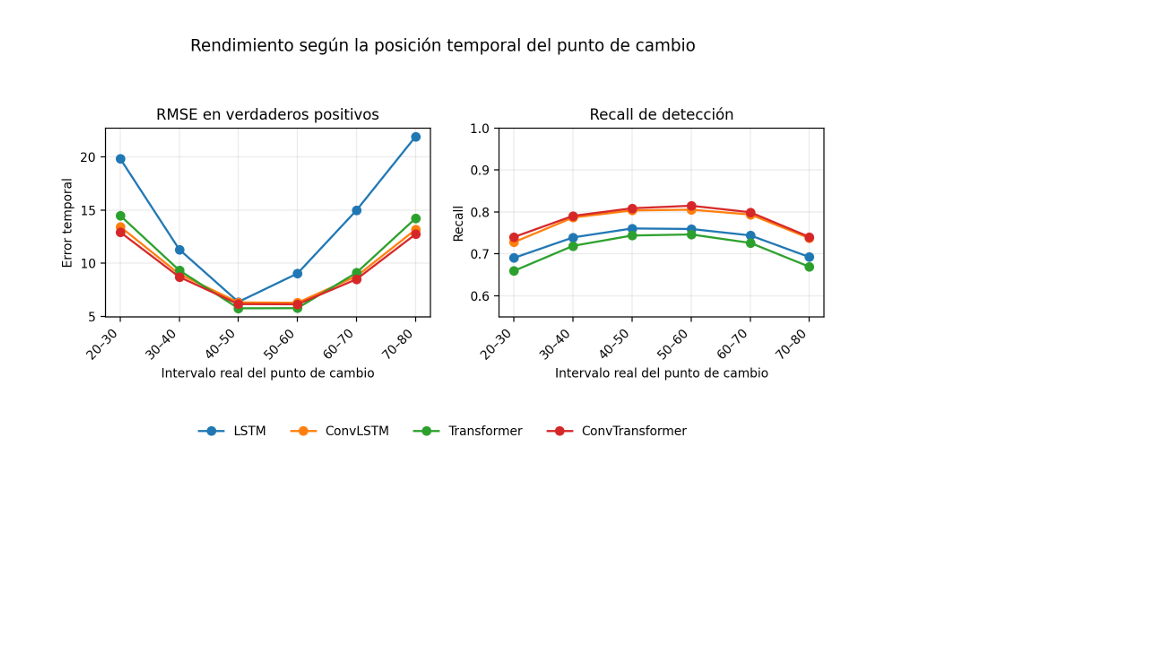
\includegraphics[width=\textwidth]{figures/section7/performance_by_changepoint_position.png}
\caption{RMSE en verdaderos positivos y sensibilidad según la posición real ($L=100$). Los cambios centrales son más favorables; cerca de los extremos, uno de los segmentos aporta menos contexto.}
\label{fig:cp-position}
\end{figure}

Los cambios centrales se localizan mejor que los cercanos a los extremos. Cuando $\tau$ está entre 40 y 60, ambos segmentos contienen suficiente contexto. En los intervalos 20--30 y 70--80, uno de los regímenes dispone de pocas observaciones y el RMSE aumenta. La forma en U aparece en todas las arquitecturas y es más marcada para LSTM. Este resultado sugiere que la longitud efectiva de cada segmento es una variable de dificultad que debe estratificarse en futuros experimentos.

\subsection{Resultado exploratorio del Protocolo A}

Cuando la presencia de cambio está garantizada, ConvTransformer obtiene MAE 7.20 y RMSE 11.63; LSTM, 7.72 y 11.71; Transformer, 7.87 y 12.37; y CNN--LSTM, 8.71 y 12.58. El orden difiere del Protocolo B: LSTM es competitivo en localización simple, pero empeora al añadir la decisión binaria. Esto muestra que localizar una frontera sabiendo que existe no equivale a detectar y localizar bajo una hipótesis nula de trayectoria homogénea.

\section{Discusión integrada}

\subsection{Compromiso entre falsas alarmas, detección y localización}

\begin{figure}[htbp]
\centering
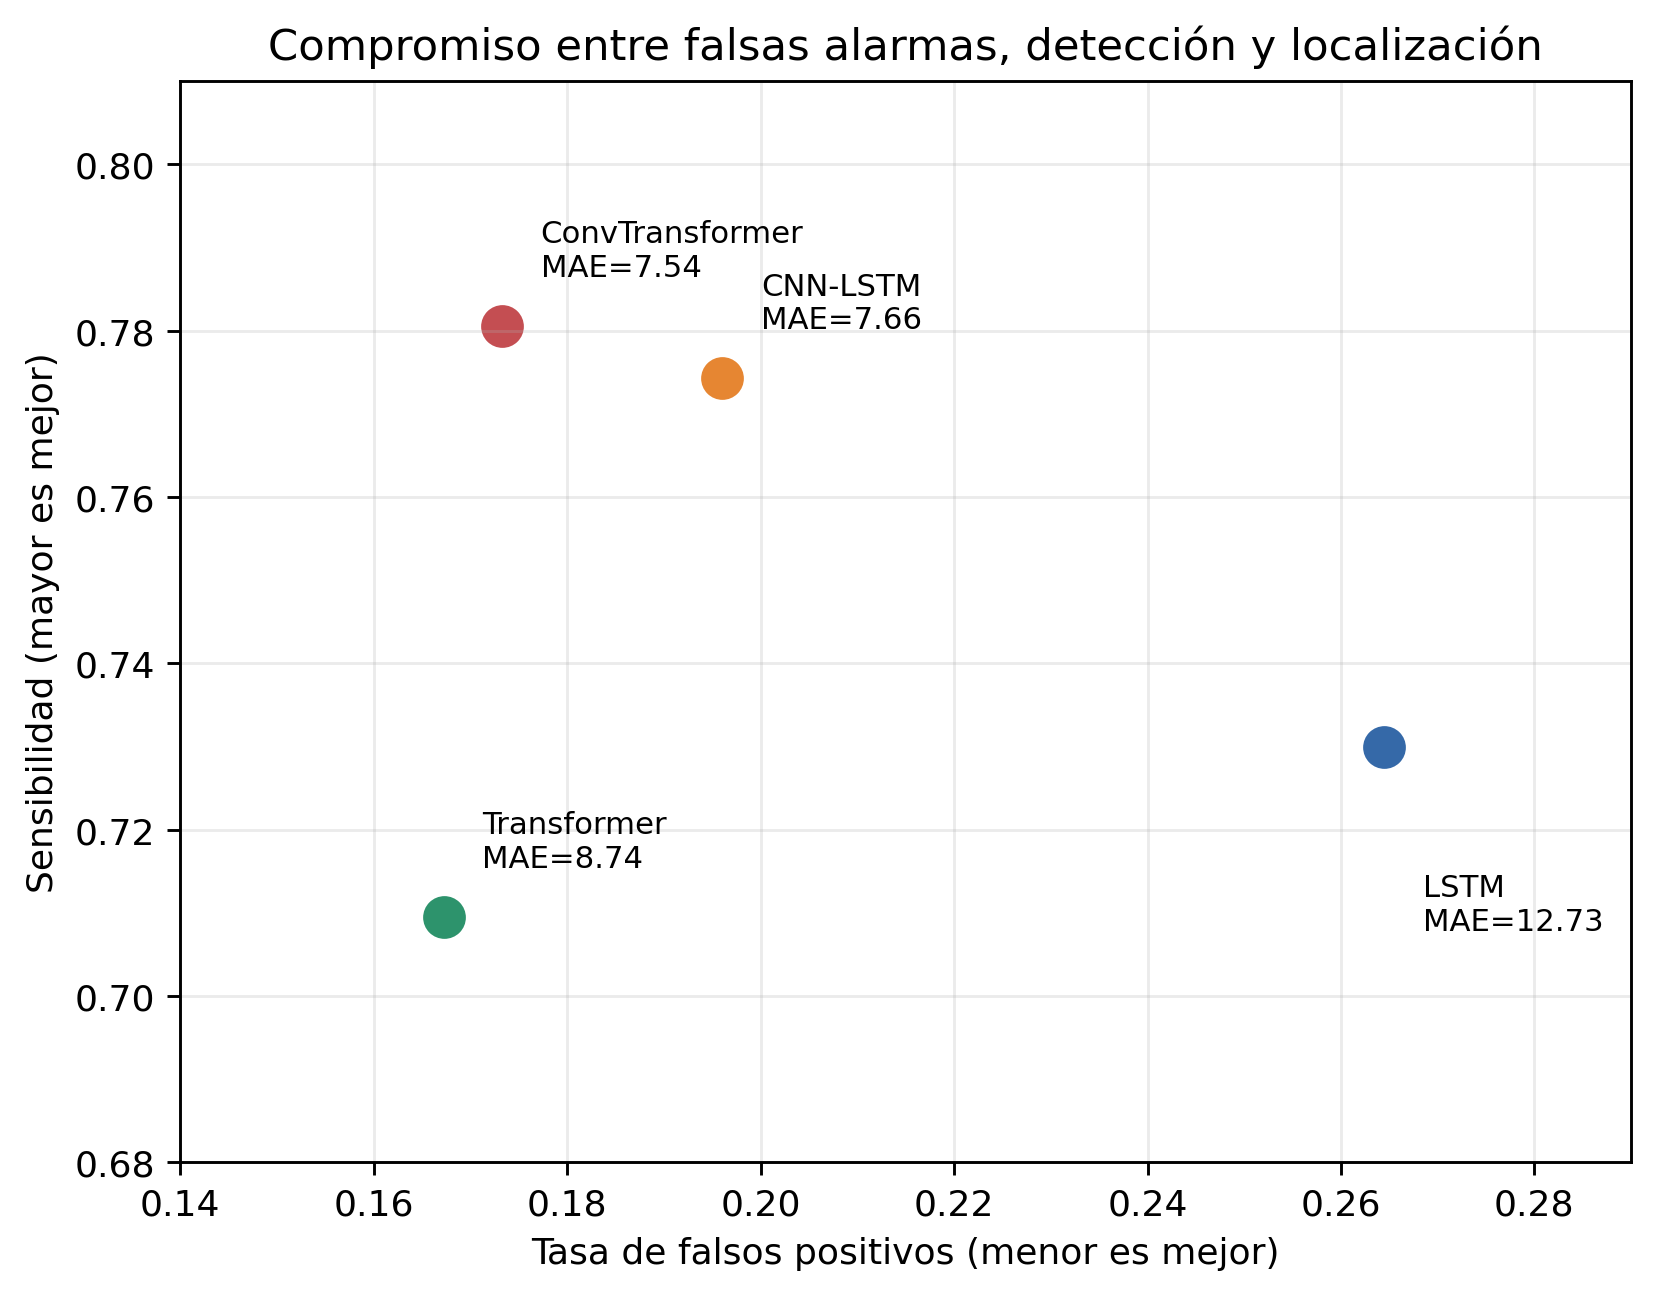
\includegraphics[width=0.86\textwidth]{figures/revised/compromiso_deteccion_localizacion.png}
\caption{Relación entre FPR, sensibilidad y MAE. La región preferible se encuentra hacia arriba y a la izquierda, con MAE pequeño.}
\label{fig:tradeoff}
\end{figure}

La Figura~\ref{fig:tradeoff} evita reducir el problema a una única clasificación. Transformer se desplaza hacia una FPR baja, pero pierde sensibilidad. CNN--LSTM conserva más cambios reales con mayor FPR. ConvTransformer ocupa la posición más equilibrada en la ejecución disponible. LSTM presenta simultáneamente FPR alta y MAE elevado.

Esta lectura coincide con la necesidad, destacada en la literatura de segmentación, de separar detección y caracterización local \cite{argun2021classification,requena2023pointwise,seckler2024changepoint}. Sin embargo, el presente experimento no reproduce RANDI ni el método de incertidumbre de Seckler y Metzler. Las referencias sirven para situar la motivación y las alternativas, no para reclamar una comparación directa de rendimiento.

\subsection{Qué información parecen aprovechar las redes}

El mejor comportamiento de las arquitecturas convolucionales es compatible con la hipótesis de que la frontera deja firmas locales en $\Delta x(t)$. Los filtros dilatados integran ventanas de varias escalas y pueden responder a cambios de persistencia o intermitencia. La atención añade una comparación global entre regiones. No obstante, esta interpretación es inferencial: sin mapas de activación, ablaciones ni datos con factores controlados, no se puede afirmar qué estadístico interno utiliza la red.

El análisis por modelo aporta evidencia indirecta. ATTM y SBM producen falsas alarmas incluso sin concatenación, lo que indica que la no estacionariedad y la heterogeneidad interna son rasgos relevantes. FBM genera dificultades cuando la transición exige reconocer un cambio de correlación. CTRW y LW forman pares favorables, posiblemente por el contraste entre pausas y vuelos persistentes. Estas explicaciones concuerdan con las propiedades de la Tabla~\ref{tab:model-properties}, pero deben contrastarse con experimentos que emparejen $\alpha$ y ruido.

\subsection{Extensiones exploratorias ConvTransformer-v3}
\label{sec:convtransformer-v3-exploratory}

ConvTransformer-v2 se mantiene como configuración principal consolidada. A partir de ella se prepararon dos variantes de diagnóstico destinadas a estudiar por separado la representación de entrada y la supervisión temporal. La selección entre variantes se planteó exclusivamente sobre validación; no se generaron métricas de test para estos ensayos.

\paragraph{ConvTransformer-v3a: entrada multicanal.}
La primera variante sustituye la entrada unicanal por seis canales calculados a partir de los incrementos observados: incrementos estandarizados por trayectoria, valor absoluto, cuadrado, varianza local con ventana cinco, media local del valor absoluto y producto con retardo uno. Todos conservan la longitud temporal $L-1$. Su construcción no consulta la etiqueta binaria, la posición verdadera de la frontera ni la identidad de los modelos generadores; por tanto, no introduce fuga de información supervisada. La finalidad es proporcionar descriptores locales explícitos de amplitud, variabilidad y dependencia de corto alcance.

\paragraph{ConvTransformer-v3b: etiquetas suaves.}
La segunda variante mantiene exactamente la entrada multicanal de v3a y modifica solo la supervisión de \texttt{cp\_dist}. En lugar de una etiqueta puntual, utiliza una distribución discreta centrada en la posición verdadera $k$:
\begin{equation}
 y^{(\sigma)}_j=
 \frac{\exp\!\left[-(j-k)^2/(2\sigma^2)\right]}
 {\sum_{\ell\in\mathcal K}\exp\!\left[-(\ell-k)^2/(2\sigma^2)\right]},
 \qquad j\in\mathcal K,
 \label{eq:soft-labels-v3b}
\end{equation}
donde $\mathcal K$ contiene las posiciones admisibles. Esta supervisión penaliza menos una predicción cercana a la frontera que otra situada muy lejos. No altera la entrada ni la cabeza binaria; en las trayectorias sin cambio, la pérdida de localización continúa anulada mediante el peso muestral.

Los ensayos disponibles corresponden a validación preliminar con semilla 42, subconjuntos reducidos y, para v3b, anchuras $\sigma=1$ y $\sigma=2$. La sensibilidad observada al umbral y la ausencia de una evaluación final controlada impiden afirmar una mejora respecto de v2. Las variantes ConvTransformer-v3a y ConvTransformer-v3b se documentan como extensiones exploratorias orientadas a analizar la representación de entrada y la supervisión de la localización. No se interpretan como sustitución del resultado principal de ConvTransformer-v2 sin una evaluación completa y controlada.

\subsection{Amenazas a la validez}

\paragraph{Validez interna.} Las pérdidas, los criterios de selección y las rejillas de umbral difieren entre arquitecturas. El número de parámetros tampoco está igualado. Por tanto, el efecto de arquitectura está confundido con decisiones de entrenamiento.

\paragraph{Variabilidad de optimización.} Se conserva una ejecución principal por arquitectura y se dispone de cinco repeticiones adicionales únicamente para ConvTransformer-v2 bajo un entrenamiento reducido. Este análisis detecta convergencias degeneradas en tres semillas, pero no estima todavía la dispersión del protocolo completo ni permite contrastar estadísticamente ConvTransformer con CNN--LSTM. Las diferencias pequeñas entre arquitecturas no deben presentarse como concluyentes.

\paragraph{Validez del generador.} Modelo y exponente cambian simultáneamente; los segmentos se normalizan; y el conjunto es sintético. La red puede aprender regularidades específicas del simulador o artefactos de concatenación. El generador binario completo debe incorporarse al repositorio.

\paragraph{Validez externa.} Todas las trayectorias son unidimensionales, solo se consideran longitudes 100 y 200 y cada señal contiene como máximo un cambio. Datos experimentales incluyen localización heteroscedástica, trayectorias truncadas, estados repetidos y múltiples transiciones.

\paragraph{Comparación con el estado del arte.} Se ejecutó una baseline PELT sobre las mismas particiones, pero su representación mediante energía y valor absoluto constituye solo una referencia clásica elemental. No se reprodujeron RANDI, AnDi-ELM ni otros métodos participantes con el protocolo original de AnDi. En consecuencia, la ventaja observada frente a PELT no establece un nuevo estado del arte ni permite afirmar que ConvTransformer supere los resultados publicados del reto.

\subsection{Reproducibilidad y redacción científica}

Una memoria reproducible debe registrar versión de \texttt{andi-datasets}, versiones de TensorFlow y NumPy, dispositivo, semillas, comandos de generación, tiempo de entrenamiento y archivos de configuración. Los cuadernos actuales documentan gran parte de la arquitectura, pero la información debe concentrarse en tablas y no depender de rutas locales. El repositorio del proyecto está disponible en \url{https://github.com/SoulaimanDev/changepoint-anomalous-diffusion} \cite{chair2026changepoint}; constituye una fuente de implementación y trazabilidad, pero no sustituye las referencias científicas.

La redacción de esta versión evita atribuir relevancia matemática a operaciones aritméticas elementales. Los tamaños de los conjuntos se expresan en tablas o en prosa. Las ecuaciones aisladas se reservan para definiciones, modelos y funciones de pérdida que vuelven a utilizarse en el análisis.

\section{Conclusiones y trabajo futuro}

Este trabajo estudia la detección y localización de una transición en trayectorias sintéticas de difusión anómala. El problema se formula como aprendizaje multitarea sobre incrementos normalizados: una salida estima la presencia de cambio y otra distribuye probabilidad sobre las posiciones admisibles. La evaluación separa trayectorias homogéneas y segmentadas, lo que evita interpretar un error de detección como si fuera únicamente un error temporal.

En la comparación de arquitecturas para $L=100$, ConvTransformer presenta el mejor compromiso global: F1 de 0.7990, sensibilidad de 0.7806, FPR de 0.1732 y MAE de localización de 7.537 muestras. CNN--LSTM obtiene resultados cercanos, especialmente en localización. Transformer minimiza la FPR, pero su sensibilidad es menor. LSTM funciona como referencia recurrente y muestra mayor dificultad en el protocolo binario.

Al fijar ConvTransformer y extender la longitud a 200, F1 alcanza 0.8440 y FPR desciende a 0.0943. Aunque el MAE absoluto aumenta a 9.376 muestras, el nMAE disminuye de 0.0754 a 0.0469. El desglose matricial es más informativo que estas medias: CTRW$\to$FBM, CTRW$\to$ATTM y ATTM$\to$FBM concentran fallos, mientras que las transiciones con LW presentan errores bajos. Debido a los cambios de lote, ponderación y umbral, esta comparación es diagnóstica y no aísla el efecto causal de $L$.

La dificultad no se distribuye uniformemente. Las trayectorias ATTM generan más falsas alarmas; FBM y SBM participan en transiciones con FNR o errores elevados; y los cambios centrales se localizan mejor que los próximos a los extremos. Estos patrones son compatibles con heterogeneidad interna, correlación de largo alcance y no estacionariedad, respectivamente.

La baseline PELT alcanzó F1 0.5302 y MAE de 16.32 muestras entre los verdaderos positivos. Su rendimiento confirma que una segmentación cuadrática sencilla sobre energía y amplitud absoluta no basta para representar todas las transiciones estudiadas. Esta comparación es interna y no equivale a reproducir AnDi, RANDI o AnDi-ELM.

El estudio de cinco semillas para ConvTransformer-v2 bajo entrenamiento reducido reveló una inestabilidad relevante: tres ejecuciones convergieron hacia una decisión casi siempre positiva. La media de F1, $0.6469 \pm 0.0363$, resulta insuficiente para describir este fallo; la FPR de $0.6974 \pm 0.4144$ ofrece una imagen más fiel. Este resultado no invalida la ejecución principal, realizada con más datos y otro presupuesto, pero impide extrapolar su rendimiento sin nuevas repeticiones completas.

Las conclusiones deben formularse con prudencia. La comparación de las cuatro arquitecturas mezcla pérdidas, presupuestos de parámetros y criterios de selección diferentes. La variabilidad solo se ha medido para ConvTransformer en un régimen reducido y la comparación con métodos publicados no reproduce sus protocolos. Por ello, ConvTransformer es la mejor configuración observada en la ejecución principal, no una arquitectura universalmente superior.

Las prioridades para continuar el estudio son:
\begin{enumerate}
  \item repetir ConvTransformer-v2 y las arquitecturas de referencia con al menos cinco semillas bajo el protocolo completo y un presupuesto común;
  \item separar cambio de modelo, cambio de exponente y cambio conjunto;
  \item comparar posiciones, incrementos brutos e incrementos normalizados;
  \item ampliar la comparación clásica con una baseline por ventanas, otras características para PELT y un método específico de difusión anómala;
  \item ampliar el estudio a más longitudes con hiperparámetros idénticos, estratificar por nivel de ruido y considerar múltiples puntos de cambio;
  \item completar la ablación de ConvTransformer-v3a y v3b exclusivamente sobre validación y evaluar en test solo la variante congelada;
  \item calibrar probabilidades y explotar la entropía o dispersión de \texttt{cp\_dist};
  \item validar sobre trayectorias experimentales o simulaciones fenomenológicas del segundo reto AnDi.
\end{enumerate}

\appendix

\section{Pseudocódigo de generación sintética}
\label{app:generation-pseudocode}

El siguiente esquema resume la construcción de las particiones sin reproducir detalles dependientes de una implementación concreta. Sea $\Mset=\{\mathrm{ATTM},\mathrm{CTRW},\mathrm{FBM},\mathrm{LW},\mathrm{SBM}\}$ y sea $L_{\min}$ la longitud mínima permitida para cada segmento.

\begin{quote}
\small
\begin{enumerate}
  \item Inicializar las particiones de entrenamiento, validación y prueba con semillas independientes.
  \item Construir las 20 transiciones ordenadas $(M_1,M_2)$ tales que $M_1,M_2\in\Mset$ y $M_1\neq M_2$.
  \item Para cada partición y cada transición:
  \begin{enumerate}
    \item muestrear $\tau\in\{L_{\min},\ldots,L-L_{\min}\}$;
    \item muestrear los exponentes dentro de los intervalos admisibles de $M_1$ y $M_2$;
    \item simular y estandarizar ambos segmentos de acuerdo con el protocolo;
    \item trasladar el segundo segmento para mantener continuidad en $\tau$;
    \item concatenar los segmentos, calcular los incrementos y guardar $(X,c=1,\tau,M_1,M_2,\alpha_1,\alpha_2)$.
  \end{enumerate}
  \item Para el Protocolo B, generar además trayectorias homogéneas de longitud $L$ con un único modelo $M\in\Mset$ y guardar $(X,c=0,M)$, sin asignar una posición de cambio.
  \item Comprobar el equilibrio entre clases, los conteos por transición y la separación de semillas entre particiones.
\end{enumerate}
\end{quote}

El pseudocódigo explicita que el orden de los modelos forma parte de la etiqueta experimental y que la posición $\tau$ solo existe para $c=1$. El código ejecutable y la organización de los experimentos se mantienen en el repositorio citado en la sección de generación de datos.

\section{Ejemplos cualitativos de ConvTransformer-v2}
\label{app:qualitative-examples}

\begin{figure}[H]
\centering
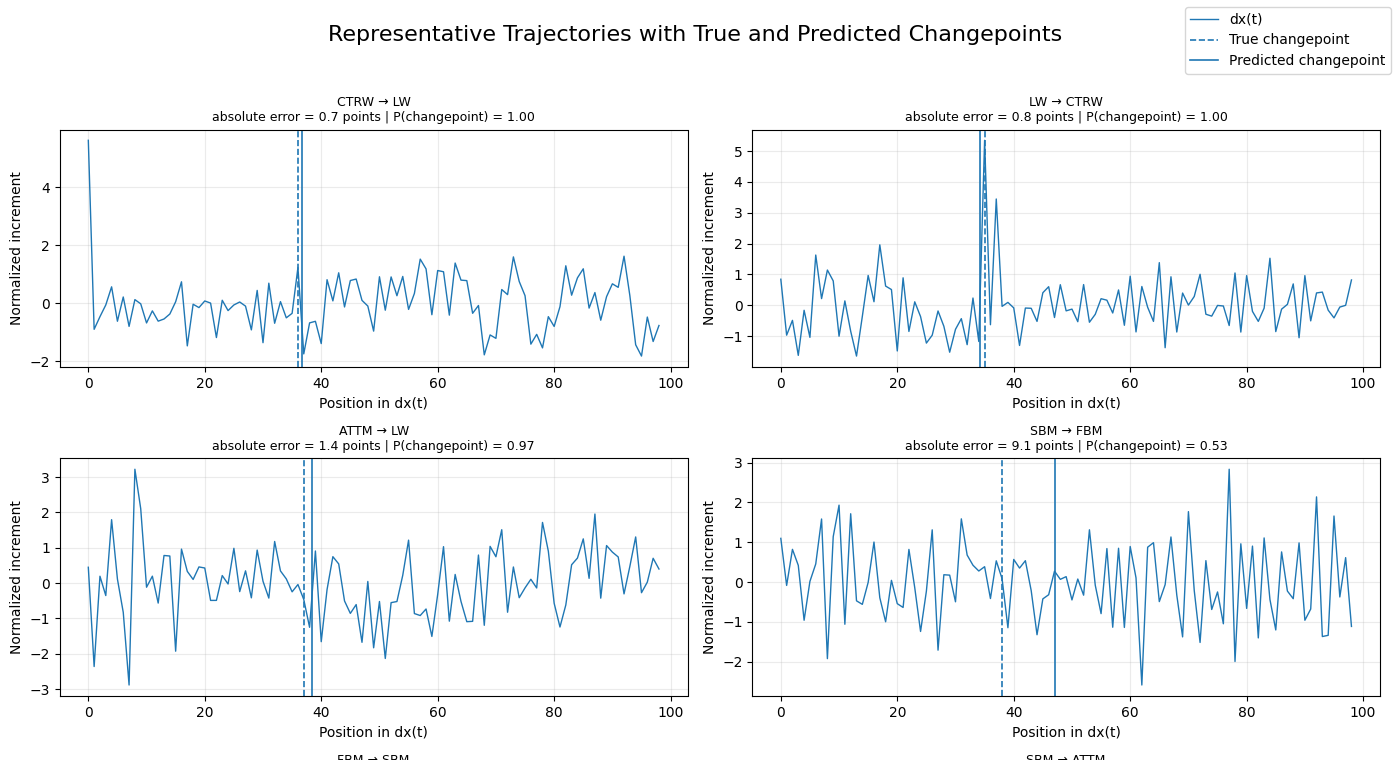
\includegraphics[width=\textwidth]{figures/revised/convtransformer_ejemplos_cualitativos.png}
\caption{Cuatro trayectorias positivas del test de ConvTransformer-v2. La línea discontinua representa la frontera verdadera y la línea continua, la estimación temporal. CTRW$\to$LW, LW$\to$CTRW y ATTM$\to$LW ilustran localizaciones próximas; SBM$\to$FBM muestra que una probabilidad de detección intermedia puede coexistir con un error temporal mayor.}
\label{fig:convtransformer-qualitative}
\end{figure}

Estas visualizaciones no sustituyen las métricas agregadas ni se utilizan para seleccionar el modelo. Su función es mostrar que detección y localización son tareas relacionadas pero distintas: una trayectoria puede recibir una probabilidad positiva razonable y, aun así, presentar una frontera estimada varios instantes lejos de la real.

\section{Protocolo propuesto de ajuste de hiperparámetros}
\label{app:tuning}

El ajuste confirmatorio debe separar selección de arquitectura, calibración del umbral y evaluación final. Se propone dividir la validación en \emph{validación de ajuste} y \emph{validación de calibración}, o utilizar validación cruzada interna. El conjunto de prueba permanece cerrado hasta congelar la configuración.

Todas las arquitecturas deben recibir el mismo presupuesto, por ejemplo 50 ensayos de búsqueda aleatoria o bayesiana. La búsqueda aleatoria es una referencia sólida cuando solo algunos hiperparámetros dominan el rendimiento \cite{bergstra2012random}. El criterio puede ser multiobjetivo: maximizar F1 y minimizar $\mathrm{MAE}_{\mathrm{all}}$. Si se requiere un único modelo, la regla de desempate debe fijarse antes de observar la prueba, por ejemplo: maximizar F1 sujeto a FPR $\leq0.20$ y, entre candidatos, minimizar MAE.

\begin{table}[htbp]
\centering
\footnotesize
\begin{tabularx}{\textwidth}{p{3.2cm}Y}
\toprule
\textbf{Grupo} & \textbf{Espacio propuesto} \\
\midrule
Común & tasa de aprendizaje $10^{-5}$--$3\cdot10^{-3}$ en escala logarítmica; lote $\{128,256,512\}$; \emph{dropout} $[0,0.4]$; peso negativo $[1,2.5]$; $\lambda_{\mathrm{loc}}\in[0.5,2]$ \\
LSTM & 1--3 capas; 64--256 unidades por capa \\
CNN--LSTM & 32--128 filtros; núcleos $\{3,5,7\}$; 1--3 bloques; dilataciones; 1--2 capas LSTM \\
Transformer & $d_{\mathrm{model}}\in\{64,96,128\}$; cabezas $\{2,4,8\}$ compatibles; 1--4 bloques; FFN 128--512 \\
ConvTransformer & espacio Transformer más 1--3 bloques convolucionales, núcleo $\{3,5,7\}$ y dilatación \\
\bottomrule
\end{tabularx}
\caption{Espacio de ajuste recomendado.}
\label{tab:tuning-space}
\end{table}

Después de elegir hiperparámetros, el umbral se calibra para todos los modelos sobre la misma rejilla $\{0,0.01,\ldots,1\}$ y con la misma utilidad. La configuración final se reentrena con cinco semillas. Deben reportarse media, desviación estándar e intervalo de confianza de F1, FPR, FNR, MAE y RMSE. También deben registrarse parámetros, tiempo y memoria para separar precisión de coste computacional.

\section{Correspondencia entre archivos y denominación}

Los nombres de archivo originales conservan la etiqueta \texttt{convlstm}. En el texto se utiliza CNN--LSTM porque la implementación contiene Conv1D seguidas de LSTM y no una celda ConvLSTM. Esta correspondencia permite reproducir los cuadernos sin mantener una denominación arquitectónica imprecisa.

\clearpage
\bibliographystyle{unsrt}
\bibliography{references_revisadas}

\end{document}
